% Copyright © 2018, Loïc Grobol <loic.grobol@gmail.com>
% This document is available under the terms of the Creative Commons Attribution 4.0 International License (CC BY 4.0) (https://creativecommons.org/licenses/by/4.0/)

\RequirePackage{xparse}
\RequirePackage{shellesc}
% Settings
\NewDocumentCommand\myname{}{Loïc Grobol}
\NewDocumentCommand\mylab{}{Lattice / ALMAnaCH}
\NewDocumentCommand\pdftitle{}{Introduction à la fouille de textes}
\NewDocumentCommand\mymail{}{loic.grobol@gmail.com}
\NewDocumentCommand\titlepagetitle{}{\pdftitle}
\NewDocumentCommand\docdate{}{2019}
\NewDocumentCommand\conference{}{M1 Plurital}

\documentclass[hyperref={unicode}, xcolor={svgnames}, french]{beamer}
\usetheme[sectionpage=progressbar,
          subsectionpage=progressbar,
          progressbar=frametitle]{metropolis}
    \definecolor{accent}{RGB}{51, 34, 136}
    \setbeamercolor{alerted text}{fg=accent}
    \makeatletter
        \setlength{\metropolis@progressinheadfoot@linewidth}{1pt}
    \makeatother
    % FIXME: not pretty and footnotes are still too big
    \let\footnoterule\relax  % No footnote rule, push down footnote

% TODO: update these to the last version
% 9-Highlights colour palette from [Paul Tol's technical note](https://personal.sron.nl/~pault/data/colourschemes.pdf)
\definecolor{highlight0}{RGB}{51, 34, 136}    % Deep blue
\definecolor{highlight1}{RGB}{136, 204, 238}  % Clear blue
\definecolor{highlight2}{RGB}{68, 170, 153}   % Teal
\definecolor{highlight3}{RGB}{17, 119, 51}    % Forest green
\definecolor{highlight4}{RGB}{153, 153, 51}   % Khaki
\definecolor{highlight5}{RGB}{221, 204, 119}  % Beige
\definecolor{highlight6}{RGB}{204, 102, 119}  % Pink
\definecolor{highlight7}{RGB}{136, 34, 85}    % Purple
\definecolor{highlight8}{RGB}{170, 68, 153}   % Violet

% Alternative navy blue for ⩽4 palettes
\definecolor{highlighta}{RGB}{68, 118, 170}  % Navy blue

% Use non-standard fonts
\usefonttheme{professionalfonts}
\setsansfont[BoldFont={Fira Sans SemiBold}, ItalicFont={Fira Sans Book Italic}]{Fira Sans Book}
\setmonofont[Scale=0.9]{Fira Mono}

% Fix missing glyphs in Fira by delegating to polyglossia/babel
\usepackage{newunicodechar}
\newunicodechar{ }{~}   % U+202F NARROW NO-BREAK SPACE
\newunicodechar{ }{ }  % U+2009 THIN SPACE

% Notes on left screen
% \usepackage{pgfpages}
% \setbeameroption{show notes on second screen=left}


\usepackage{polyglossia}
	\setmainlanguage{french}
    \setotherlanguage{english}

    % PATCH: fix spacing in monospaced text
    \usepackage{xpatch}
    \makeatletter
        \xapptocmd\ttfamily{\nofrench@punctuation}{}{}
    \makeatother

\usepackage{amsfonts,amssymb}
\usepackage{amsmath,amsthm}
\usepackage{mathtools}	% AMS Maths service pack
	\newtagform{brackets}{[}{]}	% Pour des lignes d'équation numérotées entre crochets
	\mathtoolsset{showonlyrefs, showmanualtags, mathic}	% affiche les tags manuels (\tag et \tag*) et corrige le kerning des maths inline dans un bloc italique voir la doc de mathtools
	\usetagform{brackets}	% Utilise le style de tags défini plus haut
\usepackage{lualatex-math}

\usepackage[math-style=french]{unicode-math}
	\setmathfont{Libertinus Math}
\usepackage{newunicodechar}
	\newunicodechar{√}{\sqrt}
\usepackage{mleftright}


\usepackage{tabu}
\usepackage{booktabs}
\usepackage{siunitx}
\usepackage{multicol}
\usepackage{ccicons}
\usepackage{bookmark}
\usepackage{caption}
    \captionsetup{skip=1ex}

\usepackage{csquotes}
\usepackage{tikz}
	\NewDocumentCommand{\textnode}{O{}mm}{\tikz[remember picture, baseline=(#2.base), inner sep=0pt]{\node[#1] (#2) {#3};}}
    \NewDocumentCommand{\mathnode}{O{}mm}{\tikz[remember picture, baseline=(#2.base), inner sep = 0pt]{\node[#1] (#2) {$\displaystyle #3$};}}
	\tikzset{
		alt/.code args={<#1>#2#3}{%
		\alt<#1>{\pgfkeysalso{#2}}{\pgfkeysalso{#3}} % \pgfkeysalso doesn't change the path
		},
        invisible/.style={opacity=0, fill opacity=0},
		visible on/.style={alt={<#1>{}{invisible}}}
	}
    \usepackage{forest}
    \usepackage{tkz-graph}
    \usepackage[beamer, markings]{hf-tikz}
    \usepackage{tikz-3dplot}
    \usepackage{pgfplots}
        % Due to pgfplots meddling with pgfkeys, we have to redefine alt here.
        \pgfplotsset{
    		alt/.code args={<#1>#2#3}{%
    		\alt<#1>{\pgfkeysalso{#2}}{\pgfkeysalso{#3}} % \pgfkeysalso doesn't change the path
    		},
    	}
        \pgfplotsset{compat=1.15}
        \pgfplotsset{colormap={SRON}{rgb255=(61,82,161) rgb255=(255,250,210) rgb255=(174,28,62)}}

    \usetikzlibrary{matrix}
    \usetikzlibrary{shapes, shapes.geometric}
    \usetikzlibrary{decorations.pathreplacing}
	\usetikzlibrary{positioning, calc, intersections}
    \usetikzlibrary{fit}
    \usetikzlibrary{backgrounds}

    % Do evil things with soft path
    % From <https://tex.stackexchange.com/a/301364/8547>
    \makeatletter
        \def\@appendnamedsoftpath#1{%
            \pgfsyssoftpath@getcurrentpath\@temppatha
            \expandafter\let\expandafter\@temppathb\csname tikz@intersect@path@name@#1\endcsname
            \expandafter\expandafter\expandafter\def\expandafter\expandafter\expandafter\@temppatha\expandafter\expandafter\expandafter{\expandafter\@temppatha\@temppathb}%
            \pgfsyssoftpath@setcurrentpath\@temppatha
        }
        \def\@appendnamedpathforactions#1{%
            \pgfsyssoftpath@getcurrentpath\@temppatha
            \expandafter\let\expandafter\@temppathb\csname tikz@intersect@path@name@#1\endcsname
            \expandafter\def\expandafter\@temppatha\expandafter{\csname @temppatha\expandafter\endcsname\@temppathb}%\usepackage{tikz-3dplot}

            \let\tikz@actions@path\@temppatha
        }

        \tikzset{
            use path for main/.code={%
                \tikz@addmode{%
                    \expandafter\pgfsyssoftpath@setcurrentpath\csname tikz@intersect@path@name@#1\endcsname
                }%
            },
            append path for main/.code={%
                \tikz@addmode{%
                    \@appendnamedsoftpath{#1}%
                }%
            },
            use path for actions/.code={%
                \expandafter\def\expandafter\tikz@preactions\expandafter{\tikz@preactions\expandafter\let\expandafter\tikz@actions@path\csname tikz@intersect@path@name@#1\endcsname}%
            },
            append path for actions/.code={%
                \expandafter\def\expandafter\tikz@preactions\expandafter{\tikz@preactions
                \@appendnamedpathforactions{#1}}%
            },
            use path/.style={%
                use path for main=#1,
                use path for actions=#1,
            },
            append path/.style={%
                append path for main=#1,
                append path for actions=#1
            }
        }
    \makeatother

    % TikZ externalisation
    \usetikzlibrary{external}
    % Create the `tikzpics/` folder if it does not exist
    \ShellEscape{mkdir -p tikzpics}
    % Only externalise pictures on demand (to avoid messing up with metropolis theme)
    \tikzset{
        external/export=false,
        external/prefix=tikzpics/
    }
    \tikzexternalize

\usepackage{minted}
	\usemintedstyle{lovelace}
	\setminted{autogobble, fontsize=\scriptsize, tabsize=2}
	\setmintedinline{fontsize=auto}

\usepackage[style=authoryear, block=ragged, doi=false, isbn=false]{biblatex}
    \AtEveryBibitem{
        \ifentrytype{online}
        {} {
            \iffieldequalstr{howpublished}{online}
            {
                \clearfield{howpublished}
            } {
                \clearfield{urlyear}\clearfield{urlmonth}\clearfield{urlday}
            }
        }
    }

	\addbibresource{biblio.bib}

% Compact bibliography style
\setbeamertemplate{bibliography item}[text]

\AtEveryBibitem{
    \clearfield{series}
    \clearfield{pages}
    \clearlist{publisher}
    \clearname{editor}
    \clearlist{location}
}
\renewcommand*{\bibfont}{\tiny}

\usepackage{hyperxmp}	% XMP metadata

\usepackage[type={CC},modifier={by},version={4.0}]{doclicense}

\usepackage{todonotes}
\let\todox\todo
\renewcommand\todo[1]{\todox[inline]{#1}}

\title{\titlepagetitle}
\author{\textbf{\myname} (\mylab)}
\institute{}
\date{\conference\\\docdate}

\titlegraphic{\ccby}

% Tikz styles

% Schémas de tâches
\tikzset{
    >=stealth,
    hair lines/.style={line width = 0.05pt, lightgray},
    data/.style={draw, ellipse},
    program/.style={draw, rectangle},
    accent on/.style={alt={<#1>{draw=accent, text=accent, thick}{draw}}},
    true scale/.style={scale=#1, every node/.style={transform shape}},
    highlight/.style={color=highlight#1}
}

% Styles des heatmap pour les moyennes
\pgfplotsset{
    meanheatmap/.style={
        colorbar, colormap name=SRON,
        view={0}{90},
        samples=100,
        domain=0:1,
        min=0, max=1,
        xlabel={$P$},
        ylabel={$R$},
    }
}

% Commands spécifiques
\NewDocumentCommand\shorturl{ O{https} O{://} m }{%
    \href{#1#2#3}{\nolinkurl{#3}}%
}

\DeclarePairedDelimiter\norm{\lVert}{\rVert}
\DeclarePairedDelimiter\abs{\lvert}{\rvert}
\DeclarePairedDelimiterX\compset[2]{\lbrace}{\rbrace}{#1\,\delimsize|\,#2}
\DeclarePairedDelimiterX\innprod[2]{\langle}{\rangle}{#1\,\delimsize|\,#2}

\DeclareMathOperator*\argmax{argmax}

% Easy column vectors \vcord{a,b,c} ou \vcord[;]{a;b;c}
% Here be black magic
\ExplSyntaxOn
	\NewDocumentCommand{\vcord}{O{,}m}{\vector_main:nnnn{p}{\\}{#1}{#2}}
	\NewDocumentCommand{\tvcord}{O{,}m}{\vector_main:nnnn{psmall}{\\}{#1}{#2}}
	\seq_new:N\l__vector_arg_seq
	\cs_new_protected:Npn\vector_main:nnnn #1 #2 #3 #4{
		\seq_set_split:Nnn\l__vector_arg_seq{#3}{#4}
		\begin{#1matrix}
			\seq_use:Nnnn\l__vector_arg_seq{#2}{#2}{#2}
		\end{#1matrix}
	}
\ExplSyntaxOff

\DeclareMathOperator{\TF}{TF}
\DeclareMathOperator{\IDF}{IDF}

\ExplSyntaxOn
    \DeclareExpandableDocumentCommand\eval{m}{\fp_eval:n{#1}}
\ExplSyntaxOff


% ██████   ██████   ██████ ██    ██ ███    ███ ███████ ███    ██ ████████
% ██   ██ ██    ██ ██      ██    ██ ████  ████ ██      ████   ██    ██
% ██   ██ ██    ██ ██      ██    ██ ██ ████ ██ █████   ██ ██  ██    ██
% ██   ██ ██    ██ ██      ██    ██ ██  ██  ██ ██      ██  ██ ██    ██
% ██████   ██████   ██████  ██████  ██      ██ ███████ ██   ████    ██


\begin{document}
\pdfbookmark[2]{Title}{title}

\begin{frame}[plain]
	\titlepage
\end{frame}

\lecture{Introduction à la fouille de textes}{2019-01-15}
\begin{frame}{Informations pratiques}
    \begin{description}[*]
        \item[Où] Salle Benveniste, ILPGA, 9 Rue des Bernardins, 75005 Paris
        \item[Quand] Le lundi de 13h30 à 15h30 (voir le calendrier de Paris 3 pour les dates)
        \item[Contact] \shorturl[mailto][:]{loic.grobol@gmail.com}
        \item[Web] {\shorturl{loicgrobol.github.io/intro-fouille-textes}}
    \end{description}
\end{frame}

\begin{frame}{Organisation}
    \begin{description}[*]
        \item[Poly] À lire d'une fois sur l'autre :\\
                    {\footnotesize\shorturl[https]{loicgrobol.github.io/intro-fouille-textes/poly/poly.pdf}}
        \item[Cours] Exemples, exercices, expérimentations, explications
        \item[Évaluation] en contrôle continu
            \begin{description}
                \item[Partiel] en semaine 13 → \SI{50}{\percent}
                \item[Projet] → \SI{50}{\percent}
            \end{description}
    \end{description}
\end{frame}

\begin{frame}{Projet final}
    « Utiliser des programmes d'apprentissage artificiel pour une tâche de classification de textes »
    \begin{itemize}
        \item Définir le sujet
        \item Constituer le corpus de travail
        \item Transformation du texte en données utilisables par Weka
        \item Expérimentations
        \item Compte-rendu
    \end{itemize}
\end{frame}

\begin{frame}{Weka ?}
    Une suite de logiciels pour l'apprentissage artificiel avec une interface graphique
    \begin{itemize}
        \item \shorturl{www.cs.waikato.ac.nz/ml/weka}
        \item À installer dès que possible sur votre machine
        \item Si possible, venir avec votre PC portable pour pouvoir suivre les expérimentations en cours
    \end{itemize}
\end{frame}

% ██ ███    ██ ████████ ██████   ██████  ██████  ██    ██  ██████ ████████ ██  ██████  ███    ██
% ██ ████   ██    ██    ██   ██ ██    ██ ██   ██ ██    ██ ██         ██    ██ ██    ██ ████   ██
% ██ ██ ██  ██    ██    ██████  ██    ██ ██   ██ ██    ██ ██         ██    ██ ██    ██ ██ ██  ██
% ██ ██  ██ ██    ██    ██   ██ ██    ██ ██   ██ ██    ██ ██         ██    ██ ██    ██ ██  ██ ██
% ██ ██   ████    ██    ██   ██  ██████  ██████   ██████   ██████    ██    ██  ██████  ██   ████


\section*{Introduction}

\begin{frame}{La fouille de données}
    Tout commença dans les années 90…
    \begin{itemize}
        \item Généralisation des ordinateurs personnels
        \item Augmentation de leurs capacités de mémorisation et de traitement
        \item[→] Il devient possible de traiter rapidement de grandes quantités d'informations
    \end{itemize}
    Le terme \alert{fouille de données} désigne l'ensemble des techniques permettant de prendre des décisions pertinentes à partir de l'analyse de données massives.
\end{frame}

\begin{frame}{La fouille de données}
    Intéressant et rentable
    \begin{itemize}
        \item Pour les banques et les assurances
            \begin{itemize}
                \item[→] Fiabilité d'un crédit, d'une garantie…
            \end{itemize}
        \item Pour la médecine
            \begin{itemize}
                \item[→] Efficacité d'un traitement, propagation d'une épidémie…
            \end{itemize}
        \item Pour la vente et le marketing
            \begin{itemize}
                \item[→] Cibler des publicités, étudier un marché…
            \end{itemize}
        \item …
    \end{itemize}
\end{frame}

\begin{frame}{Particularités innovantes}
    Par rapport à l'IA traditionnelle, on privilégie
    \begin{itemize}
        \item \alert{La masse de données} plutôt que les compétences expertes
        \item \alert{Les méthodes numériques} plutôt que symboliques
        \item Une démarche \alert{inductive} plutôt que déductive
            \begin{itemize}
                \item i.e. on part de nos observations pour faire des hypothèses plutôt que l'inverse
            \end{itemize}

    \end{itemize}
    Et cette tendance se généralise depuis à l'ensemble des domaines de l'informatique.

    À lire : \citetitle{church2011pendulum} \parencite{church2011pendulum}
\end{frame}

\begin{frame}{La fouille de textes}
    Applications de la fouille de données au TAL et vice-versa pour le traitement des données linguistiques massives.

    \begin{itemize}
        \item Le web 2.0 se démocratise au même moment
        \item C'est une formidable source de données linguistiques
        \item Mais elles sont en général spontanées, donc plus \alert{irrégulières} qu'auparavant
    \end{itemize}

    Et le TAL traditionnel, et en particulier
    \begin{itemize}
        \item Automates
        \item Grammaires formelles
        \item Représentations logiques
    \end{itemize}
    est moins bien équipé pour les traiter
\end{frame}

\begin{frame}{Un changement de paradigme}
    En fouille de textes, par rapport au TAL traditionnel
    \begin{itemize}
        \item On privilégie les \alert{analyses de surface}
        \item On s'appuie sur la \alert{quantité des données} pour compenser leur hétérogénéité
        \item On réduit les ambitions : pas question d'accéder au sens profond des textes
    \end{itemize}

    L'objectif est de traiter efficacement quelques \alert{tâches} précises et limitées.
\end{frame}

\begin{frame}{Sommaire}
    La suite de ce cours est articulée en deux parties
    \begin{itemize}
        \item Les tâches élémentaires de la fouille de textes
             \begin{itemize}
                 \item Qu'est-ce qu'une tâche ?
                 \item Quelles sont les tâches élémentaires ?
                 \item Combiner des tâches élémentaires
                 \item Ressources linguistiques pour la fouille de textes
                 \item Mesures de qualité des systèmes de fouille de textes
             \end{itemize}
        \item Une tâche particulière : la classification de textes
            \begin{itemize}
                \item Généralités sur la classification par apprentissage artificiel
                \item Algorithmes d'apprentissage de classification
                \item Utiliser Weka pour construire des classifieurs
            \end{itemize}
    \end{itemize}
\end{frame}

% ████████  █████   ██████ ██   ██ ███████ ███████
%    ██    ██   ██ ██      ██   ██ ██      ██
%    ██    ███████ ██      ███████ █████   ███████
%    ██    ██   ██ ██      ██   ██ ██           ██
%    ██    ██   ██  ██████ ██   ██ ███████ ███████

\section{Les tâches élémentaires de la fouille de textes}

\subsection{Notion de tâche}

\begin{frame}{Introduction}
    On traite du concept de \textit{tâche} au sens de l'informatique : spécification d'un programme qui mime une compétence humaine précise.

    \begin{itemize}
        \item Définition très large
            \begin{itemize}
                \item[→] « Tenir une conversation par écrit en se faisant passer pour un être humain » convient
            \end{itemize}
        \item En pratique on a \alert{des ambitions plus modestes}
        \item Mais on est encore loin de les satisfaire !
         \begin{itemize}
             \item Notre mesure du succès est « s'approcher le plus possible d'une solution de référence validée par un humain »
         \end{itemize}
    \end{itemize}
 \end{frame}

\begin{frame}{Caractérisation}
    \begin{itemize}
        \item Chaque tâche a une visée applicative précise et autonome
        \item Elle est caractérisée par ses \alert{entrées}, ses \alert{sorties} et les \alert{ressources} auxquelles elle fait appel
    \end{itemize}

    \begin{figure}
        \tikzset{external/export=true}
        \begin{tikzpicture}
            \node[data] (in) {Entrée};
            \node[program, right=1cm of in, text width=10ex] (prog) {Programme réalisant la tâche};
            \node[data, right=1cm of prog] (out) {Résultat};
            \draw[->] (in) -- (prog);
            \draw[->] (prog) -- (out);
        \end{tikzpicture}
    \end{figure}

    On peut considérer chaque tâche comme une \alert{boîte noire} : la façon dont le programme fonctionne ne nous intéresse pas ici.
\end{frame}

\begin{frame}{Quelques exemples de tâches}
    \begin{enumerate}
        \item Détecter les spams dans un ensemble d'emails
        \item Trouver dans le catalogue d'une bibliothèque de ouvrages qui traitent de l'art macabre au XVème siècle
        \item Trouver un site internet qui vend des ordinateurs portables sans système d'exploitation
        \item Déterminer le nom du héros et des principaux protagonistes d'un texte narratif
        \item Découper la transcription d'un discours en parties thématiques
        \item Déterminer les symptômes présentés par un patient à partir d'un rapport clinique
        \item Repérer dans un ensemble de tweets ceux qui sont sarcastiques ou ironiques
    \end{enumerate}
\end{frame}

\begin{frame}[fragile]{Schéma général d'une tâche}
    \begin{figure}
        \tikzset{external/export=true}
        \begin{tikzpicture}
            \node[ellipse, accent on=2] (in) {Entrée};
            \node[right=1cm of in, text width=10ex, accent on=3] (prog) {Programme réalisant la tâche};
            \node[ellipse, accent on=2, right=1cm of prog] (out) {Résultat};
            \node[ellipse, accent on=2, below=1cm of prog] (res) {Ressources};
            \draw[->] (in) -- (prog);
            \draw[->] (prog) -- (out);
            \draw[->] (res) -- (prog);
        \end{tikzpicture}
        \caption{Schéma général d'une tâche}
    \end{figure}
    \only<2->{
    Dans ce schéma
        \begin{itemize}
            \item<2-> Les \alert<2>{données} sont figurées par des ellipses.
            \item<3-> Le \alert<3>{programme} réalisant la tâche est figuré par un rectangle.
        \end{itemize}
    }
\end{frame}

\begin{frame}{Entrées ou ressources ?}
    Pour savoir si un élément est l'un ou l'autre, le critère qu'on retiendra en pratique est la \alert{mutabilité}
    \begin{itemize}
        \item Une ressource est une donnée stable qui n'est pas modifiée entre deux exécutions du programme
        \item Une donnée d'entrée change à chaque exécution du programme
    \end{itemize}
\end{frame}

\begin{frame}{Exemples}
    Pour les tâches suivantes, identifier entrées et sorties et proposer des ressources
    \begin{enumerate}
        \item Détecter les spams dans un ensemble d'emails
        \item Déterminer le nom du héros et des principaux protagonistes d'un texte narratif
        \item Découper la transcription d'un discours en parties thématiques
        \item Repérer dans un ensemble de tweets ceux qui sont sarcastiques ou ironiques
        \item Déterminer les symptômes présentés par un patient à partir d'un rapport clinique
    \end{enumerate}
\end{frame}

% ██████   ██████  ███    ██ ███    ██ ███████ ███████
% ██   ██ ██    ██ ████   ██ ████   ██ ██      ██
% ██   ██ ██    ██ ██ ██  ██ ██ ██  ██ █████   ███████
% ██   ██ ██    ██ ██  ██ ██ ██  ██ ██ ██           ██
% ██████   ██████  ██   ████ ██   ████ ███████ ███████

% TODO: add exemples/exercises
\begin{frame}{Données}
    On peut regrouper grossièrement les données utilisées en fouille de texte dans trois catégories
    \begin{itemize}
        \item Les données tabulaires
        \item Les textes bruts
        \item Les documents semi-structurés
    \end{itemize}
\end{frame}

\begin{frame}{Données tabulaires}
    \begin{figure}
        \includegraphics<1>[width=\textwidth, height=0.75\textheight, keepaspectratio]{pics/tab_weka.png}
        \includegraphics<2>[width=\textwidth, height=0.4\textheight, keepaspectratio]{pics/tab_weka.png}
        \caption{Données tabulaires dans Weka}
    \end{figure}
    \alt<1>{
        \vspace{-1\baselineskip}
        {\tiny Exemple Weka \texttt{weater.numeric} : peut-on jouer au tennis aujourd'hui ?}
    }{
        C'est le type de données traditionnellement utilisé en fouille de données
        \begin{itemize}
            \item L'ordre des lignes est arbitraire
            \item L'ordre des colonnes est arbitraire, sauf éventuellement pour la dernière
        \end{itemize}
    }
\end{frame}

\begin{frame}[fragile=singleslide]{Textes bruts}
    \begin{figure}
        \begin{minted}{text}
            et comment est-ce qu'on fait une omelette est-ce que vous
            pourriez m'expliquer
            comment on fait une omelette ?
            ah une omelette oui bien sûr
            je casse des oeufs
            oui oui
            je les mets dans un récipient
            je mets du sel et du poivre directement
            je bats bon je prépare ma poêle je mets du beurre hein ?
        \end{minted}
        \caption{Exemple de texte brut}
    \end{figure}
    \vskip0pt plus 1fill
    {\tiny Extrait du corpus ANCOR \parencite{muzerelle2013ANCOR}}
\end{frame}

\begin{frame}{Textes bruts}
    \alert{Tous} les caractères représentables sont susceptibles d'en faire partie
    \begin{figure}
        
\includegraphics[width=\textwidth, height=0.8\textheight, keepaspectratio]{pics/raw_emoji.png}
        \caption{Texte brut avec caractères spéciaux}
    \end{figure}
    \vskip0pt plus 1fill
    {\tiny @Biolojical@twitter : \shorturl{twitter.com/biolojical/status/949344635310059520}}
\end{frame}

\begin{frame}[fragile=singleslide]{Documents semi-structuré}
    Cas typique : XML et HTML
    \begin{figure}
        \begin{minted}{xml}
            <table>
                <tr><th>produit</th><th>marque</th><th>prix en euros</th></tr>
                <tr><td>ordinateur portable</td><td>truc</td><td>800</td></tr>
                <tr><td>tablette</td><td>machin</td><td>200</td></tr>
            </table>
        \end{minted}
        \caption{HTML vu comme texte brut}
    \end{figure}
    On peut le considérer comme du texte brut où chaque balise (\mintinline{xml}{<td>}, \mintinline{xml}{</tr>}…) compte comme un seul caractère.
\end{frame}

\begin{frame}[fragile=singleslide]{Documents semi-structuré}
    On peut aussi le considérer comme un arbre
    \begin{figure}
        % \tikzset{external/export=true}
        \begin{forest}
            for tree={font=\tiny}
            [\mintinline{xml}{<table>}
                [\mintinline{xml}{<tr>}
                    [\mintinline{xml}{<th>}
                        [produit]
                    ]
                    [\mintinline{xml}{<th>}
                        [marque]
                    ]
                    [\mintinline{xml}{<th>}
                        [{prix en euros}]
                    ]
                ]
                [\mintinline{xml}{<tr>}
                    [\mintinline{xml}{<td>}
                        [{ordinateur portable}]
                    ]
                    [\mintinline{xml}{<td>}
                        [truc]
                    ]
                    [\mintinline{xml}{<td>}
                        [800]
                    ]
                ]
                [\mintinline{xml}{<tr>}
                    [\mintinline{xml}{<td>}
                        [tablette]
                    ]
                    [\mintinline{xml}{<td>}
                        [machin]
                    ]
                    [\mintinline{xml}{<td>}
                        [200]
                    ]
                ]
            ]
        \end{forest}
        \caption{HTML vu comme un arbre}
    \end{figure}
\end{frame}

\begin{frame}{Documents semi-structurés}
    Et ils admettent dans certains cas des représentations supplémentaires
    \begin{figure}
        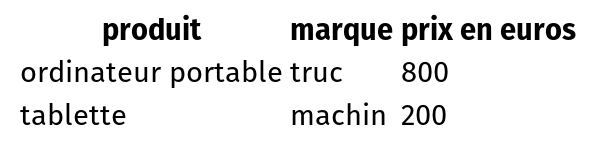
\includegraphics[width=\textwidth, height=0.8\textheight, keepaspectratio]{pics/html_firefox.png}
        \caption{Représentation du code précédent dans un navigateur}
    \end{figure}
    \vskip0pt plus 1fill
    {\tiny Représentation standard dans Mozilla Firefox \shorturl{www.mozilla.org/firefox/}}
\end{frame}

% ██████  ███████ ███████ ███████  ██████  ██    ██ ██████   ██████ ███████ ███████
% ██   ██ ██      ██      ██      ██    ██ ██    ██ ██   ██ ██      ██      ██
% ██████  █████   ███████ ███████ ██    ██ ██    ██ ██████  ██      █████   ███████
% ██   ██ ██           ██      ██ ██    ██ ██    ██ ██   ██ ██      ██           ██
% ██   ██ ███████ ███████ ███████  ██████   ██████  ██   ██  ██████ ███████ ███████


\begin{frame}{Les ressources}
    \begin{quote}
        {\only<2>{\small}Toute donnée ou programme disponible pendant l'exécution d'un programme peut être qualifiée de \emph{ressource}.}
    \end{quote}
        \only<2>{
            \begin{itemize}
                \item Listes
                    \begin{itemize}
                        \item[→] mots, caractères…
                    \end{itemize}
                \item Corpus
                \item Bases de connaissances
                    \begin{itemize}
                        \item[→] bases de données, ontologies, lexiques, wordnets…
                    \end{itemize}
                \item Programmes de pré-traitement
                    \begin{itemize}
                        \item[→] segmentation, normalisation…
                    \end{itemize}
                \item Programmes réalisant des traitements linguistiques poussés
                    \begin{itemize}
                        \item[→] lemmatisation, étiquetage morphosyntaxique…
                    \end{itemize}
            \end{itemize}
        }
\end{frame}

\begin{frame}{Quelques ressources linguistiques}
    \begin{itemize}
        \item Le Lexique Extensionnel des Formes Fléchies du Français (Lefff)
            \begin{itemize}
                \item[→] \shorturl[http]{almanach.inria.fr/~sagot/lefff.html}
            \end{itemize}
        \item La base de connaissances structurée Wikidata
            \begin{itemize}
                \item[→] \shorturl{www.wikidata.org}
            \end{itemize}
        \item Le segmenteur/étiqueteur/parser UDPipe
            \begin{itemize}
                \item[→] \shorturl{ufal.mff.cuni.cz/udpipe}
            \end{itemize}
        \item Le corpus arboré pour le français (French Treebank)
            \begin{itemize}
                \item[→] \shorturl[http]{ftb.linguist.univ-paris-diderot.fr}
            \end{itemize}
        \item Le réseau lexical JeuxDeMots
            \begin{itemize}
                \item[→] \shorturl{www.jeuxdemots.org/jdm-about.php}
            \end{itemize}
    \end{itemize}
\end{frame}

% ██████  ██████   ██████   ██████  ██████   █████  ███    ███ ███    ███ ███████ ███████
% ██   ██ ██   ██ ██    ██ ██       ██   ██ ██   ██ ████  ████ ████  ████ ██      ██
% ██████  ██████  ██    ██ ██   ███ ██████  ███████ ██ ████ ██ ██ ████ ██ █████   ███████
% ██      ██   ██ ██    ██ ██    ██ ██   ██ ██   ██ ██  ██  ██ ██  ██  ██ ██           ██
% ██      ██   ██  ██████   ██████  ██   ██ ██   ██ ██      ██ ██      ██ ███████ ███████


\begin{frame}{Programmes}
    Première option : programmes « écrits à la main »
    \begin{itemize}
        \item Reposent sur des connaissances expertes
        \item Adaptés dans des contextes stables et non-adverses
        \item Peu de robustesse aux changements et à l'hétérogénéité
        \item Dans un contexte adverse (e.g.\ spam vs.\ anti-spam), gare à la course de la reine rouge !
    \end{itemize}
    Attention : ça ne signifie pas que c'est une impasse !
    \begin{itemize}
        \item[→] FRMG (\shorturl[http]{alpage.inria.fr/frmgwiki/})
    \end{itemize}
\end{frame}

\begin{frame}[fragile=singleslide]{Programmes}
    Deuxième option : apprentissage artificiel
    \begin{figure}
        \tikzset{external/export=true}
        \begin{tikzpicture}[scale=0.9, every node/.style={transform shape}]
            \node[data] (in) {Entrée};
            \node[program, highlight=a, right=.75cm of in, text width=10ex] (prog) {Programme réalisant la tâche};
            \node[data, right=.75cm of prog] (out) {Résultat};
            \node[program, highlight=6, above=1cm of prog, text width=13ex] (progapp) {Programme d'apprentissage};
            \node[data, highlight=3, right=.75cm of progapp] (mod) {Modèle};
            \node[data, highlight=7, left=.75cm of progapp] (train) {Exemples};
            \draw[->] (in) -- (prog);
            \draw[->] (prog) -- (out);
            \draw[->] (mod) |- ($(prog.north)+(0, 0.5cm)$) -| (prog.north);
            \draw[->] (train) -- (progapp);
            \draw[->] (progapp) -- (mod);
        \end{tikzpicture}
        \caption{Schéma d'une approche par apprentissage artificiel}
    \end{figure}
    Ici le \textcolor{highlighta}{programme réalisant la tâche} est générique, mais utilise comme ressource un \textcolor{highlight3}{modèle} généré par un \textcolor{highlight6}{programme d'entraînement} à partir d'\textcolor{highlight7}{exemples} produits par des humains.
\end{frame}

\begin{frame}{Apprentissage artificiel}
    Avantages
    \begin{itemize}
        \item Peut utiliser des données d'apprentissage génériques
            \begin{itemize}
                \item[→] Permet de concentrer les besoins en connaissances expertes
            \end{itemize}
        \item En général plus robustes aux données irrégulières et à l'hétérogénéité
        \item Plus facilement transférable (e.g.\ d'une langue à une autre)
    \end{itemize}
    Inconvénients
    \begin{itemize}
        \item Parfois trop peu explicite (surtout en \textit{Deep Learning})
        \item Dépend beaucoup de la qualité des données d'entraînement
    \end{itemize}
\end{frame}

\lecture{Introduction à la fouille de textes}{2018-01-22}
\begin{frame}{Quelques exemples}
    Quelques exemples de programmes issus d'apprentissage automatique
    \begin{itemize}
        \item SEM (POS tagging, chunking, détection d'entités nommées)
            \begin{itemize}
                \item[→] \shorturl{apps.lattice.cnrs.fr/sem}
            \end{itemize}
        \item UDPipe (segmenteur/étiqueteur/parser)
            \begin{itemize}
                \item[→] \shorturl{ufal.mff.cuni.cz/udpipe}
            \end{itemize}
        \item Google translate (traduction)
            \begin{itemize}
                \item[→] \shorturl{translate.google.com}
            \end{itemize}
        \item HMTL (multi-tâches de compréhension)
            \begin{itemize}
                \item[→] \shorturl{huggingface.co/hmtl/}
            \end{itemize}
        \item @picdescbot (description d'images en langage naturel\textsuperscript{1})
            \begin{itemize}
                \item[→] \shorturl{twitter.com/picdescbot}
            \end{itemize}
    \end{itemize}
    \vskip0pt plus 1fill
    {\tiny 1. Encore plus fort : \citetitle{alishahi2017encoding} \parencite{alishahi2017encoding}}
\end{frame}

% ███████ ██    ██  █████  ██      ██    ██  █████  ████████ ██  ██████  ███    ██
% ██      ██    ██ ██   ██ ██      ██    ██ ██   ██    ██    ██ ██    ██ ████   ██
% █████   ██    ██ ███████ ██      ██    ██ ███████    ██    ██ ██    ██ ██ ██  ██
% ██       ██  ██  ██   ██ ██      ██    ██ ██   ██    ██    ██ ██    ██ ██  ██ ██
% ███████   ████   ██   ██ ███████  ██████  ██   ██    ██    ██  ██████  ██   ████


\begin{frame}{Évaluation et d'apprentissage}
    Objectif : comparer \alert{objectivement} des programmes réalisant une même tâche
    \begin{itemize}
        \item Doit se faire avec exactement les mêmes données
            \begin{itemize}
                \item Ressources et entrées !
            \end{itemize}
        \item[→] Établissement de données de référence \alert{\textit{Gold Standard}}
            \begin{itemize}
                \item[→] MetaTreebank Universal Dependencies \shorturl[http]{universaldependencies.org}
                \item[→] OntoNotes \shorturl{catalog.ldc.upenn.edu/LDC2013T19}
            \end{itemize}
        \item On met ensuite en concurrence les programmes sur ces données → challenge/shared task
            \begin{itemize}
                \item[→] CoNLL 2017 \shorturl[http]{universaldependencies.org/conll17}
                \item[→] \alert{DEFT} \shorturl{deft.limsi.fr}
            \end{itemize}
    \end{itemize}
\end{frame}

\begin{frame}{\textit{Train} et \textit{test}}
    L'évaluation d'un système ne se fait pas sur le jeu de données de développement
    \begin{itemize}
        \item Sinon une simple mémorisation suffit !
        \item On sépare le \textit{Gold Standard} en une partie \alert{\textit{train}} et une partie \alert{\textit{test}}
        \item Dans le cas d'une campagne d'évaluation, le \textit{test} est souvent tenu secret
            \begin{itemize}
                \item[→] Voir par exemple la \textit{shared task CoNLL 2017 pour un exemple sophistiqué}
            \end{itemize}
        \item[→] Valable y compris pour les programmes non-appris !
        \item On ajoute aussi parfois un ensemble dit « de développement »
        \item Classiquement \SI{80}{\percent}/\SI{10}{\percent}/\SI{10}{\percent}
    \end{itemize}
\end{frame}

\begin{frame}[fragile]{Validation croisée}
    Le découpage train/dev/test ajoute de l'objectivité et est facile à mettre en œuvre mais
    \begin{itemize}
        \item Il prive d'une partie des données → sous-performance
        \item Il induit un biais lié au découpage si celui-ci est fixe
    \end{itemize}

    Pour y limiter cet effet, on utilise parfois la méthode de validation croisée
    \begin{itemize}
        \item<1-> On découpe le corpus en $n$ parties de taille égales
        \item<2-> On utilise $n-1$ parties comme \textcolor{highlighta}{\textit{train}} et la dernière comme \textcolor{highlight6}{\textit{test}}
        \item<3-> On répète l'opération pour les $n$ combinaisons possibles
        \item<12-> On retient comme évaluation globale une moyenne des résultats
    \end{itemize}
    \begin{center}
        \tikzset{external/export=true}
        \begin{tikzpicture}[scale=0.7]
            \foreach \x in {2, ..., 11}
                \draw[alt=<\x>{fill=highlight6}{{alt=<1,12>{}{fill=highlighta}}}]
                    (\x-2, 0) -- ++(1, 0) -- ++(0, 1) -- ++(-1, 0) -- ++(0, -1) -- cycle;
        \end{tikzpicture}
    \end{center}
\end{frame}

\begin{frame}{Tâches élémentaires}
    Parmi l'ensemble des tâches, possible, certaines paraissent plus naturellement élémentaires
    \begin{itemize}
        \item Par leur relative simplicité de description
        \item Par leur capacité, en se combinant, à décrire une grande partie des autres tâches
    \end{itemize}

    Il s'agit de
        \begin{itemize}
            \item la recherche d'information (RI)
            \item la classification
            \item l'annotation
            \item l'extraction d'information (EI)
        \end{itemize}
\end{frame}

% ██████  ██
% ██   ██ ██
% ██████  ██
% ██   ██ ██
% ██   ██ ██


\subsection{La recherche d'information}

\begin{frame}[fragile=singleslide]{Recherche d'information}
    La \emph{Recherche d'Information} est la tâche consistant à trouver dans un corpus des documents \alert{pertinents} étant donnée une requête
    \begin{itemize}
        \item « Trouver dans le catalogue d'une bibliothèque de ouvrages qui traitent de l'art macabre au XVème siècle »
        \item « Trouver un site internet qui vend des ordinateurs portable sans système d'exploitation »
    \end{itemize}
    \begin{figure}
        \tikzset{external/export=true}
        \begin{tikzpicture}[true scale=0.80]
            \node[data, highlight=4] (in) {Requête};
            \node[program, right=1cm of in, text width=15ex] (prog) {Programme de RI};
            \node[data, right=1cm of prog] (out) {documents};
            \node[data, below=.6cm of prog, highlight=1] (res) {Corpus};
            \draw[->] (in) -- (prog);
            \draw[->] (prog) -- (out);
            \draw[->] (res) -- (prog);
        \end{tikzpicture}
    \end{figure}
    \vskip-1ex
    \begin{itemize}
        \item Le \textcolor{highlight1}{corpus} est une ressource obligatoire
        \item La \textcolor{highlight4}{requête} n'est \emph{pas} faite en langage fortement structuré (type SPARQL)
    \end{itemize}
\end{frame}

\begin{frame}{Domaines d'application}
    Globalement tous les moteurs de recherche
    \begin{itemize}
        \item Web : Qwant, Duckduckgo, Framabee, Google…
        \item Site : tous les sites avec une fonction de recherche (e.g. sites marchands)
        \item Documentaires : en bibliothèques, archives…
        \item …
    \end{itemize}
    Mais aussi les détecteurs de similarité
    \begin{itemize}
        \item Détection de plagiat e.g.\ Compilatio (\shorturl{compilatio.net})
        \item Détection de doublons e.g.\ sur le réseau StackExchange
    \end{itemize}
    Note : avoir défini précisément ce que « pertinent » veut dire n'est pas forcément nécessaire ! Il suffit d'avoir défini un \textit{Gold}.
\end{frame}

% WARNING: Here be dragons
\begin{frame}[fragile]{Évaluation : préliminaires}
    \begin{figure}
        \tikzset{external/export=true}
        \begin{tikzpicture}[fill opacity=0.5, text opacity=1,
                            alt=<1>{true scale=0.9}{true scale=0.75}]
            \draw[name path=D]
                (-6,-2) rectangle (6,2)
                node [above left] {$D$ : ensemble de tous les documents};
            \draw[alt={<1,6>{fill=highlight2, text=highlight2}{}}, name path=P]
                (-1, 0) circle [x radius=2, y radius=1, rotate=30]
                node[below left=1.3 and .15] {$P$ : documents pertinents};
            \draw[alt={<1,6>{fill=highlight4, text=highlight4}{}}, name path=R]
                (1, 0) circle [x radius=2, y radius=1.5]
                node[above right=1.5 and 0.1] {$R$ : documents retournés};
            \begin{scope}[alt=<2-4>{even odd rule}{}]
                \clip[alt=<2-3>{use path=P}{use path=R},
                      alt=<3-5>{append path=D}{}];
                \only<5>{\clip[use path=P, append path=D];}
                \path[alt={<2,5>{fill=highlight3}{}},
                      alt={<3,4>{fill=highlight6}{}},
                      alt=<2-3>{use path=R}{use path=P},
                      alt=<5>{use path=D}];
            \end{scope}
        \end{tikzpicture}
        \caption{Représentation de l'ensemble des documents}
    \end{figure}
    \only<2->{
        On définit les indicateurs suivants
        \begin{tabu}{|*{3}{X[m,c]|}}
            \hline
                & \uncover<2,3,6>{\textcolor{highlight4}{Retournés}}   & \uncover<4,5,6>{Non-retournés}\\
            \hline
            \uncover<2,4,6>{\textcolor{highlight2}{Pertinents}}    & \uncover<2,6>{\textcolor{highlight3}{Vrais positifs $P∩R$}}    & \uncover<4,6>{\textcolor{highlight6}{Faux négatifs $P\smallsetminus R$}}\\
            \hline
            \uncover<3,5,6>{Non-pertinents}    & \uncover<3,6>{\textcolor{highlight6}{Faux positifs $R\smallsetminus P$}} & \uncover<5,6>{\textcolor{highlight3}{Vrais négatifs $D\smallsetminus(P∪R)$}}\\
            \hline
        \end{tabu}
    }
\end{frame}

\begin{frame}{Évaluation}
    Les mesures d'évaluations usuelles rendent compte de façon synthétique du tableau précédent pour une expérience de RI
    \begin{description}
        \item[La précision] $P=\frac{VP}{VP+FP}$ « combien de documents retournés sont réellement pertinents ? »
        \item[Le rappel] $R=\frac{VP}{VP+FN}$ « parmi les documents pertinents, combien ont été trouvés ? »
        \item[La F-mesure] $F=2×\frac{P×R}{P+R}$ est la moyenne harmonique\textsuperscript{1} des deux précédentes
    \end{description}
    \vskip0pt plus 1fill
    {\tiny Exactement $F=\frac{2}{\frac{1}{P}+\frac{1}{R}}=2×\frac{P×R}{P+R}$}
\end{frame}

\begin{frame}[fragile=singleslide]{Exemples}
    Déterminer $P$, $R$ et $F$ dans les cas suivants
    \begin{itemize}
        \item $VP=1$, $VN=0$, $FP=1$, $FN=1$
        \item $VP=100$, $VN=50$, $FP=20$, $FN=15$
        \item \mbox{}\\
            {
                \tikzset{external/export=true}
                \begin{tikzpicture}[fill opacity=0.5, true scale=0.7, text opacity=1]
                    \draw[name path=D]
                        (-6,-2) rectangle (6,2)
                        node [above left] {$D$};
                    \draw[fill=highlight2, text=highlight2]
                        (-1.5, -0.25) node[text=black] {$15$} circle [x radius=2.5, y radius=1, rotate=20]
                        node[below left=1.1 and .15] {$P$ };
                    \draw[fill=highlight4, text=highlight4]
                        (1.5, 0) node[text=black] {$10$ }circle [x radius=2.5, y radius=1.7]
                        node[above right=1.5 and 0.5] {$R$};
                    \node at (0, 0) {$40$};
                    \node at (5.5, 1.5) {$2713$};
                \end{tikzpicture}
            }
    \end{itemize}
\end{frame}

\begin{frame}{Questions}
    \begin{enumerate}
        \item $P$, $R$ et $F$ dépendent-elles de la taille de $D$ ?
        \item Donner une méthode pour avoir à coup sûr $R=1$
        \item Donner une méthode pour avoir à coup sûr $P=1$
        \item Dans ces cas, que faut $F$ ? Et que vaudrait la moyenne arithmétique de $P$ et $R$.
    \end{enumerate}
\end{frame}

\lecture{Introduction à la fouille de textes}{2018-01-29}

\begin{frame}[fragile]{Aparté : moyennes}
    \begin{onlyenv}<1>
        \begin{figure}
            \tikzset{external/export=true}
            \begin{tikzpicture}
                \begin{axis}[meanheatmap]
                    \addplot3[surf, shader=interp]
                        {2*(x*y)/(x+y)};
                \end{axis}
            \end{tikzpicture}
        \caption{Moyenne harmonique de $P$ et $R$ : $2×\frac{P×R}{P+R}$}
        \end{figure}
    \end{onlyenv}
    \begin{onlyenv}<2>
        \begin{figure}
            \tikzset{external/export=true}
            \begin{tikzpicture}
                \begin{axis}[meanheatmap]
                    \addplot3[surf, shader=interp]
                        {(x+y)/2};
                \end{axis}
            \end{tikzpicture}
            \caption{Moyenne arithmétique de $P$ et $R$ : $\frac{P+R}{2}$}
        \end{figure}
    \end{onlyenv}
    \begin{onlyenv}<3>
        \begin{figure}
            \tikzset{external/export=true}
            \begin{tikzpicture}
                \begin{axis}[meanheatmap]
                    \addplot3[surf, shader=interp]
                        {(sqrt(x*y))};
                \end{axis}
            \end{tikzpicture}
        \caption{Moyenne géométrique de $P$ et $R$ : $√{P×R}$}
        \end{figure}
    \end{onlyenv}
    \begin{onlyenv}<4>
        \begin{figure}
            \tikzset{external/export=true}
            \begin{tikzpicture}
                \begin{axis}[meanheatmap]
                    \addplot3[surf, shader=interp]
                        {sqrt((x*x+y*y)/2)};
                \end{axis}
            \end{tikzpicture}
        \caption{Moyenne quadratique de $P$ et $R$ : $√{\frac{P²+R²}{2}}$}
        \end{figure}
    \end{onlyenv}
\end{frame}

\begin{frame}[fragile]{F-scores généralisés}
    \begin{columns}
    \alt<1>{\column{\textwidth}}{\column{0.45\textwidth}}
        \begin{figure}
            \tikzset{external/export=true}
            \begin{tikzpicture}[alt=<2>{true scale=0.5}{}]
                \begin{axis}[meanheatmap]
                    \addplot3[surf, shader=interp]
                        {(x*y*(1+0.5^2))/(y+x*0.5^2)};
                \end{axis}
            \end{tikzpicture}
        \caption{$F_β$ ($β=0.5$)}
        \end{figure}
    \only<2>{
        \column{0.45\textwidth}
        \vspace{\baselineskip}
        L'idée est de pondérer la moyenne harmonique
        \begin{align}
            F_{λ, μ}(P, R)
                &= \frac{λ+μ}{\frac{λ}{P}+\frac{μ}{R}}\\
                & (λ+μ) \frac{P×R}{λP + μR}\\
                &= \frac{λ+μ}{μ} \frac{P×R}{\underbrace{\frac{λ}{μ}}_{β²}P + R}\\
                &= (1+β²)\frac{P×R}{β²P + R}
        \end{align}
    }
    \end{columns}
    La F-mesure est simplement le cas $β=1$.
\end{frame}

%  ██████ ██       █████  ███████ ███████ ██ ███████
% ██      ██      ██   ██ ██      ██      ██ ██
% ██      ██      ███████ ███████ ███████ ██ █████
% ██      ██      ██   ██      ██      ██ ██ ██
%  ██████ ███████ ██   ██ ███████ ███████ ██ ██


\subsection{La classification}

\begin{frame}[label=classif,fragile]{Classification}
    La \emph{classification} est la tâche consistant à \alert{répartir} des données dans un ensemble de classes.
    \begin{itemize}
        \item « Détecter les spams dans un ensemble d'emails »
        \item « Repérer dans un ensemble de tweets ceux qui sont sarcastiques ou ironique »
        \item « Classer un ensemble de textes par genre littéraire »
    \end{itemize}
    \begin{figure}
        \tikzset{external/export=true}
        \begin{tikzpicture}[true scale=0.80]
            \node[data, highlight=4] (in) {Donnée};
            \node[program, right=1cm of in, text width=15ex] (prog) {Programme de classification};
            \node[data, right=1cm of prog] (out) {Classe};
            \node[data, below=.6cm of prog, highlight=8] (res) {Classes};
            \draw[->] (in) -- (prog);
            \draw[->] (prog) -- (out);
            \draw[->] (res) -- (prog);
        \end{tikzpicture}
    \end{figure}
    \begin{itemize}
        \item Les \textcolor{highlight8}{classes} sont connus à l'avance
        \item Chaque \textcolor{highlight4}{donnée} appartient à une classe.
    \end{itemize}
\end{frame}

\begin{frame}{Domaines d'application}
    \begin{itemize}
        \item Classification par type de document
            \begin{itemize}
                \item[→] DEFT 2018 tâche 1 (\shorturl{deft.limsi.fr/2018})
            \end{itemize}
        \item Classification par opinion/sentiment
            \begin{itemize}
                \item[→] DEFT 2018 tâche 2
            \end{itemize}
        \item Classification par qualité
            \begin{itemize}
                \item[→] \shorturl{www.youtube.com/watch?v=anwy2MPT5RE}
            \end{itemize}
        \item[…]
    \end{itemize}
    Ne s'applique pas qu'aux textes, mais de façon générale à tous les types de données !
    \begin{itemize}
        \item[→] Le temps permet-il de faire un tennis ? (Weka \texttt{weater.numeric})
        \item[→] Cet empan de texte est-il un groupe nominal ?
        \item[…]
    \end{itemize}
\end{frame}

\begin{frame}[fragile]{Évaluation}
    \colorlet{VP}{highlight3}
    \colorlet{VN}{highlight2}
    \colorlet{FN}{highlight4}
    \colorlet{FP}{highlight8}
    \begin{figure}
        \begin{tikzpicture}[
            table/.style={
                matrix of nodes,
                row sep=-\pgflinewidth,
                column sep=-\pgflinewidth,
                nodes={draw, text width=3ex, align=center},
                text depth=0.25ex,
                text height=1em,
                nodes in empty cells
            },
            aa/.style={alt=<3>{fill=VP}{}, alt={<4,5>{fill=VN}{}}},
            bb/.style={alt=<4>{fill=VP}{}, alt={<3,5>{fill=VN}{}}},
            cc/.style={alt=<5>{fill=VP}{}, alt={<3,4>{fill=VN}{}}},
            ab/.style={alt=<3>{fill=FN}{}, alt=<4>{fill=FP}{}, alt=<5>{fill=VN}{}},
            ac/.style={alt=<3>{fill=FN}{}, alt=<4>{fill=VN}{}, alt=<5>{fill=FP}{}},
            ba/.style={alt=<3>{fill=FP}{}, alt=<4>{fill=FN}{}, alt=<5>{fill=VN}{}},
            bc/.style={alt=<3>{fill=VN}{}, alt=<4>{fill=FN}{}, alt=<5>{fill=FP}{}},
            ca/.style={alt=<3>{fill=FP}{}, alt=<4>{fill=VN}{}, alt=<5>{fill=FN}{}},
            cb/.style={alt=<3>{fill=VN}{}, alt=<4>{fill=FP}{}, alt=<5>{fill=FN}{}},
        ]
            \matrix[table]{
                    & |(apred)| A   & |(bpred)| B   & |(cpred)| C\\
                |(atrue)| A   & |[aa]| $16$  & |[ab]| $0$   & |[ac]| $0$\\
                |(btrue)| B   & |[ba]| $0$   & |[bb]| $19$  & |[bc]| $1$\\
                |(ctrue)| C   & |[ca]| $0$   & |[cb]| $2$   & |[cc]| $15$\\
            };

            \draw [decorate, decoration={brace, amplitude=1em}, yshift=-0.5ex] (apred.north west) -- (cpred.north east) node [midway, above=1.25ex] {Classes prédites};
            \draw [decorate, decoration={brace, amplitude=1em, mirror}, xshift=-0.5ex] (atrue.north west) -- (ctrue.south west) node [midway, left=1.25ex, rotate=90, anchor=south] {Vraies classes};
        \end{tikzpicture}
        \caption{Matrice de confusion pour un problème à trois classes}
    \end{figure}
    \vspace{-1em}
    \only<2>{On calcule pour les mêmes indicateurs que pour la RI}
    \only<3>{Pour A}\only<4>{Pour B}\only<5>{Pour C}
    \only<2-5>{
        \begin{itemize}
            % TODO: dans la liste suivante ajouter les totaux pour chaque classe à chaque slide
            \item \textcolor{VP}{Vrais Positifs}
                \only<3>{$16$}\only<4>{$19$}\only<5>{$15$}
            \item \textcolor{VN}{Vrais Négatifs}
                \only<3>{$19+2+1+15=37$}
                \only<4>{$16+0+0+15=31$}
                \only<5>{$16+0+0+19=35$}
            \item \textcolor{FN}{Faux Négatifs}
                \only<3>{$0+0=0$}\only<4>{$0+1=1$}\only<5>{$0+2=2$}
            \item \textcolor{FP}{Faux Positifs}
                \only<3>{$0+0=0$}\only<4>{$0+2=2$}\only<5>{$0+1=1$}
        \end{itemize}
    }
    \only<6>{Puis pour chaque classe, $P$, $R$ et $F$ et la moyenne sur l'ensemble
        \begin{description}
            \item[macro-average] Sans pondération
            \item[micro-average] Pondérée par la taille des classes
        \end{description}
    }
\end{frame}


\begin{frame}{Exercice}
    Étant donnée la matrice de confusion précédente, déterminer précision, rappel et F-mesure pour chacune des classes, ainsi que la micro- et macro-average.
\end{frame}


% ██       █████  ██████  ███████ ██      ██      ██ ███    ██  ██████
% ██      ██   ██ ██   ██ ██      ██      ██      ██ ████   ██ ██
% ██      ███████ ██████  █████   ██      ██      ██ ██ ██  ██ ██   ███
% ██      ██   ██ ██   ██ ██      ██      ██      ██ ██  ██ ██ ██    ██
% ███████ ██   ██ ██████  ███████ ███████ ███████ ██ ██   ████  ██████

\lecture{Introduction à la fouille de textes}{2018-02-05}
\subsection{Annotation}

\begin{frame}[fragile=singleslide]{Annotation}
    L'\emph{annotation} ou \emph{étiquetage} est la tâche consistant à attribuer une étiquette à chaque élément d'un ensemble \alert{structuré}.

    \begin{itemize}
        \item « Déterminer les catégories grammaticales des mots d'une phrase »
        \item « Découper un discours en parties thématiques »
    \end{itemize}

    \begin{figure}
        \tikzset{external/export=true}
        \begin{tikzpicture}[true scale=0.80]
            \node[data, highlight=4] (in) {Donnée};
            \node[program, right=1cm of in, text width=12ex] (prog) {Programme d'annotation};
            \node[data, right=1cm of prog] (out) {Donnée annotée};
            \node[data, below=.6cm of prog, highlight=8] (res) {Ensemble des étiquettes};
            \draw[->] (in) -- (prog);
            \draw[->] (prog) -- (out);
            \draw[->] (res) -- (prog);
        \end{tikzpicture}
    \end{figure}
    \vskip-1em
    \begin{itemize}
        \item La \textcolor{highlight4}{donnée} à annoter est composée de plusieurs unités et munie d'une structure d'\alert{ordre}
        \item Chacune des unités se voit attribuer une des \textcolor{highlight8}{étiquettes} possibles, qui sont connus à l'avance
    \end{itemize}
\end{frame}

\begin{frame}{Structure et ordre}
    L'annotation se distingue de la classification par la notion de \emph{structure}.
    \begin{itemize}
        \item Les unités à annoter sont liées par des relations
            \begin{itemize}
                \item Ordre total (séquence)
                \item Ordre partiel (arbre, DAG)
                \item Arbitraires (graphe)
            \end{itemize}
        \item Les étiquettes qui leur sont attribuées dépendent de ces relations
    \end{itemize}
\end{frame}

\begin{frame}[fragile=singleslide]{Exemples}
    \begin{figure}
        \tikzset{external/export=true}
        \begin{tikzpicture}
            \matrix[matrix of nodes, anchor=base, row sep=1.5em] (m) {
                Le  & petit & chat  & est & mort\\
                DET & ADJ   & NC    & V   & ADJ\\
            };
            \foreach \x in {1, ..., 5}
                \draw[->] (m-1-\x) -- (m-2-\x);
        \end{tikzpicture}
        \caption{\emph{Part Of Speech Tagging}}
    \end{figure}
\end{frame}

\begin{frame}[fragile=singleslide]{Exemples}
    \begin{figure}
        \tikzset{external/export=true}
        \begin{tikzpicture}
            \matrix[matrix of nodes, anchor=base, row sep=1.5em] (m) {
                Le  & petit & chat  & est & mort\\
                B & I   & I   & B & B\\
            };
            \foreach \x in {1, ..., 5}
                \draw[->] (m-1-\x) -- (m-2-\x);

            \matrix[matrix of nodes, anchor=base, below=2em of m] (s){
                (   & Le    & petit & chat & )  & ( & est   & ) & (  & mort & )\\
            };
            \foreach \x/\y in {4/5, 4/6, 5/8, 5/9}
                \draw[->] (m-2-\x) -- (s-1-\y);
        \end{tikzpicture}
        \caption{\emph{Chunking}}
    \end{figure}
\end{frame}

\begin{frame}[fragile=singleslide]{Exemples}
    \begin{figure}
        \tikzset{external/export=true}
        \begin{tikzpicture}
            \tikzset{every tree node/.style={align=center,anchor=north}}
            \Tree [.S
                [.NP→\textcolor{highlighta}{sub} [.Det the ] [.N cat ] ]
                [.VP→\textcolor{highlighta}{pred} [.V sat ]
                    [.PP→\textcolor{highlighta}{mod} [.P on ]
                        [.NP [.Det the ] [.N mat ] ]
                    ]
                ]
            ]
        \end{tikzpicture}
        \caption{\textcolor{highlighta}{Étiquetage fonctionnel} d'un arbre syntaxique}
    \end{figure}
\end{frame}

\begin{frame}{Évaluation}
    Pour évaluer un étiquetage, on choisit en général de le considérer comme un problème de classification à plusieurs classes
    \begin{itemize}
        \item On considère chaque unité comme une donnée et chaque étiquette comme une classe
        \item On calcule comme précédemment $P$, $R$ et $F$
        \item On privilégie les micro-averages pour les scores globaux
    \end{itemize}
\end{frame}

\begin{frame}[fragile]{Aparté : micro-average et exactitude}
    \begin{theorem}
        Si chaque unité reçoit une unique étiquette, les micro-average de $P$, $R$ et $F$ sont égales à l'exactitude.
    \end{theorem}
    On considère la matrice de confusion suivante
    \begin{center}
        \tikzset{external/export=true}
        \begin{tikzpicture}[
            table/.style={
                matrix of nodes,
                row sep=-\pgflinewidth,
                column sep=-\pgflinewidth,
                nodes={draw, text width=3ex, align=center},
                text depth=0.25ex,
                text height=1em,
                nodes in empty cells
            },
            aa/.style={},
            bb/.style={},
            cc/.style={},
            ab/.style={},
            ac/.style={},
            ba/.style={},
            bc/.style={},
            ca/.style={},
            cb/.style={},
        ]
            \matrix[table]{
                    & |(apred)| A   & |(bpred)| B   & |(cpred)| C\\
                |(atrue)| A   & |[aa]| $aa$  & |[ab]| $ab$   & |[ac]| $ac$\\
                |(btrue)| B   & |[ba]| $ba$   & |[bb]| $bb$  & |[bc]| $bc$\\
                |(ctrue)| C   & |[ca]| $ca$   & |[cb]| $cb$   & |[cc]| $cc$\\
            };

            \draw [decorate, decoration={brace, amplitude=1em}, yshift=-0.5ex] (apred.north west) -- (cpred.north east) node [midway, above=1.25ex] {Classes prédites};
            \draw [decorate, decoration={brace, amplitude=1em, mirror}, xshift=-0.5ex] (atrue.north west) -- (ctrue.south west) node [midway, left=1.25ex, rotate=90, anchor=south] {Vraies classes};
        \end{tikzpicture}
    \end{center}
    Et on regarde le tableau !
\end{frame}

% TODO: add slides for the proof above

% ███████ ██
% ██      ██
% █████   ██
% ██      ██
% ███████ ██

\subsection{L'extraction d'informations}
\begin{frame}[fragile]{Extraction d'informations}
    L'\emph{extraction d'informations} est la tâche consistant à trouver dans un document les \alert{réponses} à des questions prédéfinies.

    \only<1>{
        \begin{itemize}
            \item « Déterminer le nom du héros et des principaux protagonistes d'un texte narratif »
            \item « Déterminer les symptômes présentés par un patient à partir d'un rapport clinique »
        \end{itemize}
    }

    \begin{figure}
        \tikzset{external/export=true}
        \begin{tikzpicture}[true scale=0.80]
            \node[data, highlight=4] (in) {Donnée};
            \node[program, right=1cm of in, text width=12ex] (prog) {Programme d'EI};
            \node[data, right=1cm of prog, highlight=6] (out) {Champs remplis};
            \node[data, below=.6cm of prog, highlight=8] (res) {Champs à remplir};
            \draw[->] (in) -- (prog);
            \draw[->] (prog) -- (out);
            \draw[->] (res) -- (prog);
        \end{tikzpicture}
    \end{figure}

    \only<2>{
        \begin{itemize}
            \item La \textcolor{highlight4}{donnée} est un texte brut ou un document semi-structuré
            \item La \textcolor{highlight6}{sortie} est un tableau qui donne la valeur de chacun des champs
            \item Les \textcolor{highlight8}{champs} \emph{peuvent} être multivalués et en nombre variable
        \end{itemize}
    }
\end{frame}

% TODO: add cites
\begin{frame}{Domaines d'application}
    Ils sont nombreux !
    \begin{itemize}
        \item Identification de protagonistes (littérature, militaire)
        \item Identification d'événement (biomédical, militaire)
        \item Fouille d'arguments
            \begin{itemize}
                \item Aide à la décision (politique)
                    \begin{itemize}
                        \item[→] IBM Watson (\textcite{slonim2014claims}, \shorturl{youtube.com/watch?v=sEf0GLvrP9U})
                    \end{itemize}
                \item Aide à la lecture (judiciaire, scientifique)
                    \begin{itemize}
                        \item[→] « Argument zoning » (\textcite{teufel2009argument}, \shorturl{www.cl.cam.ac.uk/~sht25/az.html})
                    \end{itemize}
            \end{itemize}
        \item …
    \end{itemize}
    À l'extrême, la tâche se confond avec la compréhension de document.
\end{frame}

\begin{frame}{Évaluation}
    L'idée est toujours de se comparer à une référence humaine.
    \begin{itemize}
        \item Basiquement : on compare les contenus des champs et on en déduit $P$, $R$ et $F$
        \item Plus subtilement : on peut utiliser des mesures d'adéquation entre les réponses
            \begin{itemize}
                \item[→] Une réponse peut être partiellement correcte : on pondère~!
            \end{itemize}
        \item Pour certaines tâches, on utilise des mesures spécifiques
            \begin{itemize}
                \item Pour les tâches comprenant une composante de localisation (NER, Argument Zoning), on peut appliquer des pondérations différentes à extraction et localisation
            \end{itemize}
    \end{itemize}
\end{frame}

% ██████  ███████ ██       █████  ████████ ██  ██████  ███    ██ ███████
% ██   ██ ██      ██      ██   ██    ██    ██ ██    ██ ████   ██ ██
% ██████  █████   ██      ███████    ██    ██ ██    ██ ██ ██  ██ ███████
% ██   ██ ██      ██      ██   ██    ██    ██ ██    ██ ██  ██ ██      ██
% ██   ██ ███████ ███████ ██   ██    ██    ██  ██████  ██   ████ ███████


\subsection{Relations entre tâches}
\begin{frame}<1>[label=taskrel]{Relations entre tâches}
    Les tâches présentées précédemment sont \emph{élémentaires} au sens où on peut y réduire la plupart des tâches de la fouille de texte.

    Cependant ces tâches ne sont pas complètement indépendantes les unes des autres \emph{via} des reformulations.
\end{frame}

\begin{frame}[fragile=singleslide]{La RI comme classification}
    Puisque la RI consiste à déterminer parmi un ensemble de documents lesquels sont pertinents, on peut la voir comme un problème de classification binaire.

    \begin{itemize}
        \item On répartit les documents entre les deux classes « pertinent » et « non-pertinent »
        \item La requête, qui était une donnée, devient une ressource
    \end{itemize}
    \vskip-1em
    \begin{figure}
        \tikzset{external/export=true}
        \begin{tikzpicture}[true scale=0.75]
            \node[data] (in) {Requête};
            \node[program, right=2cm of in, text width=16ex] (prog) {Programme de classification};
            \node[data, right=1.5cm of prog] (out) {Documents pertinents};
            \node[above left=0.25cm and 0.25cm of prog.north west] (ri) {RI};
            \draw ($(prog.north west)+(-1.5cm, 0.75cm)$) -- ($(prog.north east)+(1cm, 0.75cm)$) -- ($(prog.south east)+(1cm, -1.25cm)$) -- ($(prog.south west)+(-1.5cm, -1.25cm)$) -- cycle;
            \node[data, below=1.5cm of prog] (res) {Corpus};
            \draw[->] (in.south) |- ($(prog.south)-(0, 0.75cm)$) -- (prog.south);
            \draw[->] (res.west) -| ($(prog.west)-(0.75cm, 0)$) -- (prog.west);
            \draw[->] (prog) -- (out);
        \end{tikzpicture}
        \caption{La RI comme une classification}
    \end{figure}
\end{frame}

% TODO: add graphics and examples
\begin{frame}{L'annotation comme classification}
    Plusieurs stratégies sont envisageables pour conserver l'information de structure
    \begin{itemize}
        \item Voir la suite des étiquettes d'une séquence comme une seule classe.
        \item Étiqueter par classifications successives en utilisant à chaque étape l'ensemble des étiquettes précédentes comme information pour choisir l'étiquette suivante.
    \end{itemize}
\end{frame}

% TODO: add slides for EI as tagging


% ██████  ███████  ██████  ██████  ███    ███ ██████
% ██   ██ ██      ██      ██    ██ ████  ████ ██   ██
% ██   ██ █████   ██      ██    ██ ██ ████ ██ ██████
% ██   ██ ██      ██      ██    ██ ██  ██  ██ ██
% ██████  ███████  ██████  ██████  ██      ██ ██

\lecture{Introduction à la fouille de textes}{2018-02-12}
\subsection{Décomposition en tâches élémentaires}
\begin{frame}[fragile]{Décomposition en tâches élémentaires}
    Les tâches \emph{élémentaires} le sont parce qu'on peut y réduire des tâches plus complexes.

    \only<1>{
        \begin{figure}
            \tikzset{external/export=true}
            \begin{tikzpicture}[true scale=0.75]
                \node[data] (in) {Entrée};
                \node[right=1cm of in, text width=10ex, accent on=<1>] (prog) {Programme};
                \node[data, right=1cm of prog] (out) {Résultat};
                \draw[->] (in) -- (prog);
                \draw[->] (prog) -- (out);
            \end{tikzpicture}
            \caption{Schéma général d'une tâche}
        \end{figure}
        Le \alert{programme} réalisant la tâche sera ainsi composé de sous-programmes réalisant des tâches élémentaires.
    }

    \only<2>{
        \begin{figure}
            \tikzset{external/export=true}
            \begin{tikzpicture}[true scale=0.75]
                \node[data] (in1) {Entrée};
                \node[program, right=1cm of in1, text width=12ex] (prog1) {Programme élémentaire};
                \node[data, right=0.75cm of prog1] (out1) {Résultat};
                \draw[->] (in1) -- (prog1);
                \draw[->] (prog1) -- (out1);

                \node[program, right=0.75cm of out1, text width=12ex] (prog2) {Programme élémentaire};
                \node[data, right=1cm of prog2] (out2) {Résultat};
                \draw[->] (out1) -- (prog2);
                \draw[->] (prog2) -- (out2);

                \draw ($(prog1.north west)+(-0.5cm, 1cm)$) rectangle ($(prog2.south east)+(0.5cm, -1cm)$);
            \end{tikzpicture}
            \caption{Décomposition d'une tâche complexe}
        \end{figure}
    }

    \only<3>{
        \begin{figure}
            \tikzset{external/export=true}
            \begin{tikzpicture}[true scale=0.75]
                \node[data] (in1) {Entrée};
                \node[program, right=2cm of in1, text width=12ex] (prog1) {Programme élémentaire};
                \node[data, right=1cm of prog1] (out1) {Résultat};
                \draw[->] (in1) -- (prog1);
                \draw[->] (prog1) -- (out1);

                \node[program, above=1cm of out1, text width=12ex] (prog2) {Programme élémentaire};
                \node[data, right=2cm of prog2] (out2) {Résultat};
                \draw[->] (out1) -- (prog2);
                \draw[->] (prog2) -- (out2);
                \draw[->] (in1) -- ($(prog1.west)-(0.75cm, 0)$) |- (prog2.west);

                \draw ($(prog1.south west)+(-1cm, -1cm)$) rectangle ($(prog2.north east)+(1cm, 1cm)$);
            \end{tikzpicture}
            \caption{Décomposition d'une tâche complexe}
        \end{figure}
    }
\end{frame}

\begin{frame}{Exemple : les systèmes de Question/Réponse}
    Les systèmes de question/réponse fournissent des réponses factuelles à des requêtes données en langage naturel

    \begin{figure}
        \tikzset{external/export=true}
        \begin{tikzpicture}[true scale=0.75]
            \node[data, text width=15ex] (in) {« Quelle est la vitesse d'une hirondelle ? »};
            \node[program, right=1cm of in, text width=15ex] (prog) {Programme de Q/R};
            \node[data, right=1cm of prog] (out) {« \SI{60}{km/h} »};
            \node[data, below=.6cm of prog] (res) {Corpus};
            \draw[->] (in) -- (prog);
            \draw[->] (prog) -- (out);
            \draw[->] (res) -- (prog);
        \end{tikzpicture}
        \caption{Structure d'un système de Q/R}
    \end{figure}
\end{frame}

\begin{frame}[fragile]{Q/R via RI}
    % TODO: add progressive result feedback on the “Quelle est la vitesse d'une hirondelle sample question”
    % TODO: add arrow colours
    La première reformulation possible utilise un système de \alert<1>{RI}

    \begin{figure}
        \tikzset{external/export=true}
        \begin{tikzpicture}[true scale=0.55]
            \node[data, alt=<2>{highlight=6}{}] (in) {Question};
            \node[coordinate, right=1cm of in] (split) {};
            \fill[alt=<2>{highlight=6}{}] (split) circle[radius=2pt];
            \draw[alt=<2>{highlight=6, thick}{}] (in) -- (split);

            \node[program, above right=0.5cm and 1cm of split, alt=<2>{highlight=a}{}] (term) {Terminologie};
            \node[data, right=1cm of term, alt=<3>{highlight=a}{}] (words) {Mots};
            \node[program, right=1cm of words, accent on=<1>, alt=<3>{highlight=3}{}] (ri) {RI};
            \node[data, right=1cm of ri, alt=<3-4>{highlight=8}{}] (docs) {Docs};
            \node[program, right=1cm of docs, alt=<4>{highlight=3}{}] (ei) {EI};
            \node[coordinate, below right=0.5cm and 1cm of ei] (gather) {};
            \node[data, right=1cm of gather, alt=<4>{highlight=a}{}] (answer) {Réponse};
            \draw[->, alt=<2>{highlight=6, thick}{}] (split) |- (term);
            \draw[->] (term) -- (words);
            \draw[->] (words) -- (ri);
            \draw[->] (ri) -- (docs);
            \draw[->] (docs) -- (ei);
            \draw[->] (ei) -| (gather) -- (answer);

            \node[program, below right=0.5cm and 1cm of split, alt=<2>{highlight=3}{}] (classif) {Classifieur};
            \node[data, below=1cm of ei, alt=<4>{highlight=2}{}] (field) {Champs};
            \draw[->, alt=<2>{highlight=6, thick}{}] (split) |- (classif);
            \draw[->] (classif) -- (field);
            \draw[->] (field) -- (ei);

            \draw ($(split)+(-0.5cm, 2cm)$) rectangle ($(field.south east)+(1cm, -0.5cm)$);

            \node[data, below=3cm of ri, alt=<3>{highlight=2}{}] (corpus) {Corpus};
            \draw[->] (corpus) -- (ri);
        \end{tikzpicture}
        \caption{Système de Question/Réponse via Recherche d'Informations}
    \end{figure}
    \only<2->{
        \begin{itemize}
            \only<2>{
                \item \textcolor{highlight6}{La question en langage naturel} est envoyée en parallèle à \textcolor{highlighta}{un extracteur de mots-clés} et à un \textcolor{highlight3}{classifieur} qui détermine le type de la réponse attendue
            }
            \only<3>{
                \item \textcolor{highlighta}{Les mots-clés extraits} sont utilisés comme requête pour \textcolor{highlight3}{le programme de RI} qui sélectionne dans \textcolor{highlight2}{le corpus} \textcolor{highlight8}{les documents pertinents} pour répondre à la question
            }
            \only<4>{
                \item<4> \textcolor{highlight3}{Un programme d'EI} extrait des \textcolor{highlight8}{documents pertinents} le contenu des \textcolor{highlight2}{champs}, qui constituent la \textcolor{highlighta}{réponse} à la question posée
            }
        \end{itemize}
    }
\end{frame}

\begin{frame}<1>[fragile]{Q/R via base de connaissances}
    % TODO: add further overlay
    % TODO: add progressive result feedback on the “Quelle est la vitesse d'une hirondelle sample question”
    % TODO: add arrow colours
    Une autre stratégie consiste à reformuler la question en requête dans une \alert<1>{base de connaissances structurée}

    \begin{figure}
        \tikzset{external/export=true}
        \begin{tikzpicture}[true scale=0.6]
            \node[data, alt=<2>{highlight=6}{}] (in) {Question};
            \node[coordinate, right=1cm of in] (split) {};
            \draw[alt=<2>{highlight=6, thick}{}] (in) -- (split);

            \node[program, above right=0.5cm and 1cm of split, alt=<2>{highlight=a}{}] (trad) {Traduction};
            \node[data, right=1cm of trad, alt=<2-3>{highlight=3}{}] (req) {Requête};
            \node[program, right=1cm of req, alt=<3>{highlight=3}{}] (int) {Interrogation};
            \node[coordinate, below right=0.5cm and 1cm of int] (gather) {};
            \node[data, right=1cm of gather, alt=<4>{highlight=a}{}] (answer) {Réponse};
            \draw[->, alt=<2>{highlight=6, thick}{}] (split) |- (trad);
            \draw[->] (trad) -- (req);
            \draw[->] (req) -- (int);
            \draw[->] (int) -| (gather) -- (answer);

            \node[program, below=1cm of req, alt=<2>{highlight=3}{}] (ei) {EI};
            \node[data, accent on=<1>, alt=<4>{highlight=2}{}] at (int|-ei) (base) {Base};
            \draw[->] (ei) -- (base);
            \draw[->] (base) -- (int);

            \draw ($(split|-trad.north)+(-0.5cm,0.5cm)$) rectangle ($(int.east|-ei.south)+(1.25cm, -0.5cm)$);

            \node[data, below=1cm of ei, alt=<3>{highlight=2}{}] (corpus) {Corpus};
            \draw[->] (corpus.west) -- ++ (-0.25cm, 0) |- (ei.west);
        \end{tikzpicture}
        \caption{Système de Question/Réponse utilisant une base de connaissances}
    \end{figure}
    \only<2->{
        \begin{itemize}
            \item<2|only@2> \textcolor{highlight6}{La question en langue naturelle} est \textcolor{highlighta}{traduite} en une \textcolor{highlight3}{requête} dans un langage formel (SQL, SPARQL…)
        \end{itemize}
    }
\end{frame}

% TODO: add links and refs for the two deompositions

\begin{frame}{Conclusion}
    On a donc vu qu'on pouvait
    \begin{itemize}
        \item Réaliser des tâches complexes en se ramenant des tâches élémentaires
        \item Reformuler les tâches élémentaires en terme de classification
    \end{itemize}

    En pratique, on peut donc presque toujours ramener n'importe quelle tâche de fouille de texte à de la classification, on parlera donc pour celle-ci de \alert{tâche pivot}.
    \begin{itemize}
        \item[→] Attention cependant à ne pas faire cuire les pâtes comme un mathématicien…
    \end{itemize}
\end{frame}

% ██████  ███████ ██████  ██████  ███████ ███████
% ██   ██ ██      ██   ██ ██   ██ ██      ██
% ██████  █████   ██████  ██████  █████   ███████
% ██   ██ ██      ██      ██   ██ ██           ██
% ██   ██ ███████ ██      ██   ██ ███████ ███████


\section{Représentation des données}

\begin{frame}{Représentation des données}
    Étant donné que
    \begin{itemize}
        \item La classification joue en fouille de texte le rôle de tâche pivot
        \item On privilégie pour la classification des données au format tabulaire
    \end{itemize}
    Il est naturel de vouloir mettre les données à traiter sous forme tabulaire.
\end{frame}

% ███████ ████████  █████  ████████
% ██         ██    ██   ██    ██
% ███████    ██    ███████    ██
%      ██    ██    ██   ██    ██
% ███████    ██    ██   ██    ██

\subsection{Spécificités statistiques}
\begin{frame}{Loi de Zipf}
    Dans \textit{Ulysse} de James Joyce on\textsuperscript{1} observe\textsuperscript{2} que
    \begin{itemize}
        \item Le mot le plus courant apparaît \num{8000} fois
        \item Le dixième mot le plus courant apparaît \num{800} fois
        \item Le centième mot le plus courant apparaît \num{80} fois
        \item Le millième mot le plus courant apparaît \num{8} fois
    \end{itemize}

    \begin{block}{Hypothèse (Loi de Zipf)}
        La fréquence $f(n)$ du $n$-ième mot le plus fréquent d'un corpus vérifie
        \begin{equation}
            f(n) = \frac{K}{n}
        \end{equation}
        où $K$ est une constante ne dépendant que du corpus.
    \end{block}
    \vskip0pt plus 1fill
    {\tiny 1. Georges Zipf (1902-1950) dans \parencite{zipf1949human}\\2. d'après la légende}
\end{frame}

% TODO: add Ulysse répartition
% TODO: add visualisation for fat tail
\begin{frame}{Loi de Zipf : observations}
    \begin{figure}
        \tikzset{external/export=true}
        \begin{tikzpicture}
            \begin{axis}[xmin=0, ymin=0, xmax=20,
                         width=0.9\textwidth,
                         height=0.8\textheight,
                         xlabel={Rang},
                         ylabel={Fréquence d'apparition},
                         title={Loi de Zipf : $y=\frac{K}{x}$},
                         scaled ticks=false,
                         ticklabel style={/pgf/number format/.cd, 1000 sep={\,}}]
                \addplot[highlighta, domain=1:20, samples=1001] {max(8000/x, 1)};
            \end{axis}
        \end{tikzpicture}
        \caption{Courbe d'une loi de Zipf ($K=\num{8000}$)}
    \end{figure}
\end{frame}

% TODO: add cites
\begin{frame}{Loi de Zipf : observations}
    \begin{itemize}
        \item La loi de Zipf se vérifie plutôt bien expérimentalement
        \item En pratique, les répartitions observées sont de la forme $f(n)=\frac{k}{x^s}$ avec $s$ proche de $1$
        \item Ce type de distribution, dites \emph{loi de puissance} est omniprésent en statistiques (en en sciences en général)
        \item Elles font parties des distributions dites \emph{à longue traîne} (\textit{fat tail})
        \item Une autre approche due à Mandelbrot présente une généralisation de la loi de Zipf comme le résultat de contraintes d'optimalité d'utilisation d'un canal de communication.
    \end{itemize}
\end{frame}

\begin{frame}{Loi de Heaps}
    Si la loi de Zipf donne une estimation de la répartition du vocabulaire d'un corpus, la loi de Heaps est une estimation de sa diversité
    \begin{block}{Hypothèse : loi de Heaps}
        Le nombre $V$ de mots distincts dans sous-corpus de taille $M$ vérifie
        \begin{equation}
            V = K×M^β
        \end{equation}
        Où $K$ et $β$ sont des paramètres dépendant du corpus
    \end{block}
    \begin{itemize}
        \item[→] Ce $K$ n'est pas le même que pour la loi de Zipf, et $β$ n'a aucun lien avec la pondération de $F_β$
        \item[→] On parle souvent de relation \emph{types-tokens}
        \item[→] Pour l'anglais, on a $K∈[30, 100]$ et $β≈0.5$
        \item[→] Cette loi peut-elle être valable quelle que soit la taille de la collection ?
    \end{itemize}
\end{frame}

\begin{frame}[label=heapslawgraph]{Loi de Heaps}
    \begin{figure}
        \tikzset{external/export=true}
        \begin{tikzpicture}
            \begin{axis}[xmin=0, xmax=800000, ymin=0,
                         width=0.9\textwidth,
                         height=0.8\textheight,
                         xlabel={Taille de la collection},
                         ylabel={Taille du vocabulaire},
                         title={Loi de Heaps : $y=K×x^β$},
                         scaled ticks=false,
                         ticklabel style={/pgf/number format/.cd, 1000 sep={\,}}]
                \addplot[highlighta, domain=0:800000, samples=1001] {40*x^0.5};
            \end{axis}
        \end{tikzpicture}
        \caption{Courbe d'une loi de Heaps}
    \end{figure}
\end{frame}
%
% ███████ ███████  █████  ████████ ███████
% ██      ██      ██   ██    ██    ██
% █████   █████   ███████    ██    ███████
% ██      ██      ██   ██    ██         ██
% ██      ███████ ██   ██    ██    ███████


\subsection{Choix des attributs}
\begin{frame}{Choix des attributs}
    Pour pouvoir faire de la classification, il faut pouvoir mettre les données au bon format
    \begin{description}[<+->][*]
        \item[Objectif] Transformer les documents à traiter en fichiers tabulaires pour les passer à un classifieur
        \item[Problème] Quel choix d'attributs (colonnes) ?
        \item[Solution] Ça dépend des cas !
            \begin{itemize}
                \item[→] Mais on peut identifier plusieurs stratégies élémentaires (air connu)
            \end{itemize}
    \end{description}
\end{frame}

\begin{frame}[fragile=singleslide]{Caractères}
    Puisqu'un texte brut est une séquence de caractères : utilisons comme attribut la fréquence de chaque caractère

    \begin{figure}
        \begin{tabu}{*{5}{>{\ttfamily\small}X[m, c]}}
            Texte   & a & b & c & …\\
            Ulysse  & 90578 & 17848 & 27902 & …
        \end{tabu}
    \end{figure}

    \begin{itemize}
        \item Combien d'attributs par texte ?
        \item Est-ce suffisant ?
            \begin{itemize}
                \item Suffisant pour quoi ?
            \end{itemize}
    \end{itemize}
\end{frame}

\begin{frame}{$n$-grammes de caractères}
    % TODO: add corrections
    % TODO: add sources
    % TODO: add examples
    Une stratégie un peu plus raffinée est de compter non pas les caractères, mais les séquences de caractères de longueur $n$.

    Exemple : « Le petit chat est mort »

    \begin{itemize}
        \item Quels sont les unigrammes ?
        \item Quels sont les bigrammes ?
        \item Quels sont les trigrammes ?
        \item En général, pour un alphabet à $k$ caractères, combien y a-t-il de $n$-grammes ?
    \end{itemize}

    En pratique, les trigrammes peuvent suffire pour certaines applications !
    \begin{itemize}
        \item Détection du plagiat
    \end{itemize}

    Pour plus de richesse, on peut aussi utiliser des \emph{skip-grams}
\end{frame}

\lecture{Introduction à la fouille de textes}{2018-02-19}

\begin{frame}<-2>{Mots}
    Faisons \alt<1>{enfin de la}{un peu de} linguistique : comptons les mots !
    \begin{itemize}
        \item Problème : qu'est-ce qu'un mot ?
            \begin{itemize}
                \item \emph{pomme de terre} ?
                \item \emph{y a-\textbf{t}-il} ?
                \item …
            \end{itemize}
        \item On a plutôt tendance à compter les \alert{tokens}
            \begin{itemize}
                \item « Séquences de caractères comprises entre deux séparateurs »
                \item[→] Problème : qu'est-ce qu'un séparateur ? \begin{itemize}
                    \item « E-mail » vs. « Alsace–Lorraine »
                    \item « […] kiwi. Hier […] » vs. « M. Martin »
                    \item « Yann Le Bourdonnec » vs. « Félix le chat »
                \end{itemize}
                \item On délègue à un segmenteur (\emph{tokenizer})
            \end{itemize}
    \end{itemize}
\end{frame}

\begin{frame}<1>[label=wordcols]{Des mots aux colonnes}
    Objectif : utiliser les fréquences des mots comme attributs (colonnes) dans une représentation tabulaire.
    \begin{itemize}
        \item Combien de colonnes faut-il ?
\only<2->{
            \begin{itemize}
                \item[→] $K×M^β$ (loi de Heaps)
                \item Pour \emph{Ulysse}, environ \num{34000}
            \end{itemize}
        \item Il faut donc arriver à filtrer !
            \begin{itemize}
                \item Supprimer les mots vides (\emph{stop words}) : \emph{le}, \emph{à}, \emph{mais}…
                \item Ne conserver certaines catégories spécifiques à la tâche (noms, adjectifs…)
                \item Supprimer les hapax (mots n'apparaissant qu'un seule fois)
                \item[→] De façon générale, ne conserver qu'une bande de fréquence
            \end{itemize}
}
    \end{itemize}
\end{frame}

\againframe{heapslawgraph}

\againframe<2>{wordcols}

\begin{frame}[fragile]{Filtrer les hapax}
    \begin{figure}
        \tikzset{external/export=true}
        \begin{tikzpicture}
            \begin{axis}[xmin=0, ymin=0, xmax=40, ymax=15,
                         xtick=\empty,
                         ytick=\empty,
                         alt=<2>{extra y ticks={1}}{},
                         width=0.9\textwidth,
                         height=0.8\textheight,
                         xlabel={Rang},
                         ylabel={Fréquence d'apparition},
                         title={$y=\frac{K}{x}$}]
                \addplot[highlighta, domain=1:20, samples=501] {20/x};
                \addplot[highlighta, alt=<2>{dotted}{}, domain=20:40, samples=500] {1};
                \only<2>{
                    \draw[highlight6] (axis cs:0,1) -- (current axis.east|-{axis cs:0,1});
                }
            \end{axis}
        \end{tikzpicture}
        \caption{\alt<2>{Filtrage des hapax sur la c}{C}ourbe de Zipf}
    \end{figure}
\end{frame}

\againframe<2>{wordcols}

\begin{frame}[fragile=singleslide]{Filtrer une bande de fréquences}
    \begin{figure}
        \tikzset{external/export=true}
        \begin{tikzpicture}
            \begin{axis}[xmin=0, ymin=0, xmax=40, ymax=20,
                         xtick=\empty,
                         ytick={2, 15},
                         yticklabels={$a$, $b$},
                         width=0.9\textwidth,
                         height=0.8\textheight,
                         xlabel={Rang},
                         ylabel={Fréquence d'apparition},
                         title={$y=\frac{K}{x}$}]
                \addplot[highlighta, dotted, domain=1:1.33, samples=333] {20/x};
                \addplot[highlighta, domain=1.33:10, samples=333] {20/x};
                \addplot[highlighta, dotted, domain=10:40, samples=333] {max(20/x,1)};
                \draw[highlight6] (axis cs:0,15) -- (current axis.east|-{axis cs:0,15});
                \draw[highlight6] (axis cs:0,2) -- (current axis.east|-{axis cs:0,2});
            \end{axis}
        \end{tikzpicture}
        \caption{Filtrage d'une bande de fréquences sur la courbe de Zipf}
    \end{figure}
\end{frame}

\begin{frame}{Mots}
    Pour réduire encore plus le nombre de colonnes
    \begin{itemize}
        \item Lemmatiser : \{\emph{est}, \emph{était}, \emph{suis}, \emph{êtes}, \emph{furent}…\} → \emph{est}
        \item Radicaliser : \{\emph{homme}, \emph{hommes}\} → \emph{homme}
        \item Fixer un lexique \emph{a priori}
            \begin{itemize}
                \item[→] Avec les dangers que ça comporte
            \end{itemize}
    \end{itemize}

    À l'inverse, pour plus de détails, on peut utiliser des $n$-grammes de mots
    \begin{itemize}
        \item[→] Représentation plus riche, mais amplifie le problème de quantité
    \end{itemize}
\end{frame}

\begin{frame}{Traits linguistiques avancés}
    Si les ressource le permettent, on peut envisager d'autres attributs
    \begin{itemize}
        \item Avec un étiqueteur morphosyntaxique : POS, $n$-grammes de POS
        \item Avec un parser : largeur/profondeur/taille moyenne des arbres/constituants, paires gouverneur-gouverné, paires nœud-relation…
        \item Avec des analyseurs sémantiques : rôles
        \item Avec des bases de connaissances : présence de certains concepts
        \item …
    \end{itemize}
    Mais on introduit alors des dépendances vis-à-vis des ressources, ce qui multiplie les causes d'erreurs.
\end{frame}

% ███    ███ ███████  █████  ███████ ██    ██ ██████  ███████
% ████  ████ ██      ██   ██ ██      ██    ██ ██   ██ ██
% ██ ████ ██ █████   ███████ ███████ ██    ██ ██████  █████
% ██  ██  ██ ██      ██   ██      ██ ██    ██ ██   ██ ██
% ██      ██ ███████ ██   ██ ███████  ██████  ██   ██ ███████

\subsection{Valuation des attributs}
\begin{frame}[label=attrval]{Valuation des attributs}
    Avoir choisi les attributs à utiliser pour une classification ne suffit pas : encore faut-il leur donner une valeur
    \begin{description}[*]
        \item[Booléenne] Vrai/Faux ($0$/$1$) suivant que l'attribut est ou n'est pas présent dans le document
        \item[Occurrences] Le nombre $n_{i,j}$ de fois qu'apparaît l'attribut $a_j$ dans le document $t_i$
        \item[Fréquences normalisées par ligne] (ici pour la norme $1$)
            \begin{equation}
                \frac{\mathnode{freqfracnum}{n_{i,j}}}{\mathnode{freqfracden}{\sum_k n_{i,k}}}
            \end{equation}
    \end{description}
    \textbf{Note} : ici et dans la suite, on considère que toutes les colonnes sont de même nature
\end{frame}

\begin{frame}[fragile=singleslide]{Notations}
    \begin{itemize}
        \item Les textes sont notés $t_1$, $t_2$, …, $t_m$
        \item Les attributs sont notés $a_1$, $a_2$, …, $a_n$
        \item La valeur du $j$-ème attribut pour le $i$-ème texte est notée $a_{i,j}$ (ligne, colonne)
    \end{itemize}

    \begin{figure}
        \begin{tabu} to 0.9\linewidth {X[m, c]|*{4}{X[m, c]}}
                    & $a_1$     & $a_2$     & $…$ & $a_n$\\
            \hline
            $t_1$   & $a_{1,1}$ & $a_{1,2}$ & $…$ & $a_{1,n}$\\
            $t_2$   & $a_{2,1}$ & $a_{2,2}$ & $…$ & $a_{2,n}$\\
            $⋮$    & $⋮$      & $⋮$       &     & $⋮$\\
            $t_m$   & $a_{m,1}$ & $a_{m,2}$ & $…$ & $a_{m,n}$\\
         \end{tabu}
    \end{figure}
\end{frame}

\againframe{attrval}

% TODO: add cites
\begin{frame}{TF.IDF}
    On veut pouvoir pondérer l'importance d'un terme (mot, caractère, $n$-gramme…) en fonction de sa spécificité (au sens large) pour un document.

    \begin{itemize}
        \item \emph{\textbf{T}erm \textbf{F}requency $×$ \textbf{I}nverse \textbf{D}ocument \textbf{F}requency}
        \item $\TF(i,j) = n_{i,j}$ ou $\TF(i,j) = \frac{n_{i,j}}{\sum_k n_{i,j}}$
        \item
            \only<1>{
                \begin{equation}
                    \IDF(j) = \log\mleft(\frac{m}{\#\compset{i}{a_{i,j}>0}}\mright)
                \end{equation}
            }
            \only<2>{
                \begin{equation}
                    \IDF(j) = \log\frac{\overbrace{m}^{\mathclap{\text{nombre total de documents}}}}{\underbrace{\#\compset{i}{a_{i,j}>0}}_{\mathclap{\text{nombre de documents contenant $a_j$}}}}
                \end{equation}
            }
            \only<3->{$\IDF(j) = \log\frac{m}{\#\compset{i}{a_{i,j}>0}}$}
        \only<3->{
            \item Intuitivement $\IDF$ mesure la rareté d'un attribut, donc (on espère !) son informativité
            \item « Si $a_j$ est présent dans tous les textes, savoir qu'il est présent dans $t_i$ ne donne pas d'information sur $t_i$ »
            \item Permet un filtrage moins arbitraire des \emph{stop words}
            \item \alt<4>{$\log$ donne à $\IDF$ la forme d'une \emph{surprise} au sens de Shannon}{$\log$ est une façon pratique de modérer les effets de cette pondération : on devrait parler de $\log$-$\IDF$}
        }
    \end{itemize}
\end{frame}

\subsection{Représentations vectorielles et similarités}

\begin{frame}{Des sacs de mots aux vecteurs}
    Dans tout ce qui précède, on ne tient pas compte des positions relatives des termes, mais seulement de leurs nombres d'occurrences.
    \begin{itemize}
        \item Approche \emph{bag-of-words} (sac de mots)
        \item « Siobhan tue Eóghan » vs. « Eóghan tue Siobhan »…
        \begin{itemize}
            \item[→] On compte (comme d'habitude) sur la masse de données pour passer outre ce genre de problèmes
        \end{itemize}
    \end{itemize}
    En pratique on fait même plus fort
    \begin{itemize}
        \item Hypothèse d'indépendance : si $k≠ℓ$, $a_k$ et $a_ℓ$ sont indépendants
        \item On peut alors considérer chaque ligne comme un vecteur (ou un point…) d'un espace vectoriel
        \item Et accéder à la puissance de l'algèbre linéaire et de la géométrie vectorielle !
    \end{itemize}
\end{frame}

\begin{frame}{Les maths en cinq secondes : vecteurs}
    On appelle \emph{vecteur de dimension $n$} tout $n$-uplet de nombres
    \begin{equation}
        v = \vcord{v_1, ⋮, v_n}
    \end{equation}
    Si $n=2$, on peut les représenter simplement dans le plan
    \begin{figure}
        \tikzset{external/export=true}
        \begin{tikzpicture}
            \draw [help lines, xstep=1cm, ystep=1cm] (0, 0) grid (5.25, 4.25);

            \draw[->] (-0.5,0) -- (5.25, 0);
            \foreach \x in {1,...,5}
                \draw[shift={(\x, 0)}] (0pt,2pt) -- (0pt,-2pt) node[below] {\footnotesize $\x$};
            \draw[->] (0, -0.5) -- (0, 4.25);

            \foreach \y in {1,...,4}
                \draw[shift={(0,\y)}] (2pt,0pt) -- (-2pt,0pt) node[left] {\footnotesize $\y$};

            \draw (0, 0) node[below left] {\footnotesize $0$};

            \draw [->, highlighta, line width=2pt] (0,0) -- (2,3);

            \draw (1.5, 1.5) node[anchor=west] {$\textcolor{highlighta}{v}=\vcord{2,3}$};
        \end{tikzpicture}
        \caption{Vecteur en dimension $2$}
    \end{figure}
\end{frame}

\begin{frame}{Les maths en cinq secondes : vecteurs}
    On définit la \emph{somme} et le \emph{produit par un nombre} par
    \begin{equation}
        \vcord{a_1, ⋮, a_n} + \vcord{b_1, ⋮, b_n} = \vcord{a_1+b_1, ⋮, a_n+b_n}
    \end{equation}
    et
    \begin{equation}
        λ⋅\vcord{a_1, ⋮, a_n} = \vcord{λa_1, ⋮, λa_n}
    \end{equation}
    par exemple
    \begin{equation}
        \vcord{2, 7} + \vcord{1, 3} = \vcord{3, 10}
    \end{equation}
    \begin{equation}
        5⋅\vcord{3.5, -3} = \vcord{17.5, -15}
    \end{equation}
\end{frame}

\begin{frame}[fragile]{Les maths en cinq secondes : vecteurs}
    Géométriquement
    \only<1-4>{
        \begin{figure}
            \tikzset{external/export=true}
            \begin{tikzpicture}
                \draw [help lines, xstep=1cm, ystep=1cm] (0, 0) grid (5.25, 4.25);

                \draw[->] (-0.5,0) -- (5.25, 0);
                \foreach \x in {1,...,5}
                    \draw[shift={(\x, 0)}] (0pt,2pt) -- (0pt,-2pt) node[below] {\footnotesize $\x$};
                \draw[->] (0, -0.5) -- (0, 4.25);

                \foreach \y in {1,...,4}
                    \draw[shift={(0,\y)}] (2pt,0pt) -- (-2pt,0pt) node[left] {\footnotesize $\y$};

                \draw (0, 0) node[below left] {\footnotesize $0$};

                \draw [->, highlighta, line width=2pt, alt=<2-3>{invisible}{}] (0,0) -- (3,1) node[midway, above] {$v$};
                \draw [->, highlighta, line width=2pt, alt=<2-3>{}{invisible}] (1,2) -- (4,3) node[midway, above] {$v$};

                \draw [->, highlight3, line width=2pt] (0,0) -- (1,2) node[midway, above left] {$u$};

                \draw[->, highlight6, line width=2pt, alt=<3->{}{invisible}] (0,0) -- (4,3) node[midway, right] {$u+v$};
            \end{tikzpicture}
            \caption{Somme de deux vecteurs}
        \end{figure}
    }
    \only<5-7>{
        \begin{figure}
            \tikzset{external/export=true}
            \begin{tikzpicture}
                \draw [help lines, xstep=1cm, ystep=1cm] (0, 0) grid (5.25, 4.25);

                \draw[->] (-0.5,0) -- (5.25, 0);
                \foreach \x in {1,...,5}
                    \draw[shift={(\x, 0)}] (0pt,2pt) -- (0pt,-2pt) node[below] {\footnotesize $\x$};
                \draw[->] (0, -0.5) -- (0, 4.25);

                \foreach \y in {1,...,4}
                    \draw[shift={(0,\y)}] (2pt,0pt) -- (-2pt,0pt) node[left] {\footnotesize $\y$};

                \draw (0, 0) node[below left] {\footnotesize $0$};

                \draw [->, highlighta, line width=2pt, alt=<5>{}{invisible}] (0,0) -- (2,1) node[midway, above] {$v$};

                \draw[->, highlighta, line width=2pt, alt=<6>{}{invisible}] (0,0) -- (4,2) node[midway, above] {$2v$};
                \draw[->, highlighta, line width=2pt, alt=<7>{}{invisible}] (0,0) -- (1,0.5) node[above] {$0.5v$};
            \end{tikzpicture}
            \caption{produit d'un vecteur par un nombre}
        \end{figure}
    }
\end{frame}

\begin{frame}{Interprétation}
    Bien entendu, l'hypothèse d'indépendance est fausse en général
    \begin{itemize}
        \item[→] Si un texte contient \emph{main}, il est plus probable qu'il contienne également \emph{doigt}
    \end{itemize}
    Et représenter les documents par des vecteurs a ses limites
    \begin{itemize}
        \item[→] Que signifie le fait des sommer les attributs de deux documents ?
    \end{itemize}
    Mais ces approximations permettent d'utiliser une machinerie mathématique qui marche suffisamment bien en pratique.

    On est bien dans la philosophie de la fouille de textes !
\end{frame}

\begin{frame}{Similarité : exemple de travail}
    En pratique, les documents considérés auront beaucoup de colonnes
    \begin{itemize}
        \item De quelques-unes à plusieurs centaines
        \item Donc les vecteurs considérés seront de grande dimension
        \item Mais pour l'intuition on va se retreindre à la dimension $2$ : le plan
    \end{itemize}
\end{frame}

\begin{frame}[standout]
    \textit{To deal with a $14$-dimensional space, visualize a $3$-D space and say `fourteen' to yourself very loudly. Everyone does it.}

    Geoffrey Hinton
\end{frame}

\begin{frame}[fragile=singleslide]{Similarités : exemple de travail}
    On considère deux vecteurs $t_1=(v_{1,1}, … v_{1,n})$ et $t_2=(v_{2,1}, …, v_{2,n})$ représentant des documents

    Par exemple, si on utilise comme traits les fréquences de \emph{orange} et \emph{kiwi}, étant donné le fichier tabulaire suivant
    \begin{columns}
    \column{0.5\textwidth}
        \begin{figure}
            \begin{tabu} to .9\linewidth {*{3}{X[c]}}
                \texttt{t}  & \texttt{orange} & \texttt{kiwi}\\
                \hline
                \texttt{1}  & \texttt{3}      & \texttt{1}\\
                \texttt{2}  & \texttt{1}      & \texttt{2}\\
            \end{tabu}
        \end{figure}

        On aura $t_1=\tvcord{3, 1}$ et $t_2=\tvcord{1, 2}$
    \column{0.5\textwidth}
        \begin{figure}
            \tikzset{external/export=true}
            \begin{tikzpicture}[true scale=0.8]
                \draw [help lines, xstep=1cm, ystep=1cm] (0, 0) grid (5.25, 4.25);

                \draw[->] (-0.5,0) -- (5.25, 0);
                \foreach \x in {1,...,5}
                    \draw[shift={(\x, 0)}] (0pt,2pt) -- (0pt,-2pt) node[below] {\footnotesize $\x$};
                \draw[->] (0, -0.5) -- (0, 4.25);

                \foreach \y in {1,...,4}
                    \draw[shift={(0,\y)}] (2pt,0pt) -- (-2pt,0pt) node[left] {\footnotesize $\y$};

                \draw (0, 0) node[below left] {\footnotesize $0$};

                \draw [->, highlighta, line width=2pt] (0,0) -- (3,1) node[midway, above] {$t_1$};
                \draw [->, highlight3, line width=2pt] (0,0) -- (1,2) node[midway, above left] {$t_2$};
            \end{tikzpicture}
            \caption{Exemple de travail}
    \end{figure}
\end{columns}
\end{frame}

% TODO: overlay equation uncover ?
% TODO: distances comparisons (particularly minkovsky) : show distorted diagrams ?
% TODO: for all examples → connect to real-world examples with word frequences
\begin{frame}[fragile]{Distance de Manhattan}
    \begin{block}{Définition (distance de Manhattan)}
        On appelle \emph{distance de Manhattan} entre $t_1$ et $t_2$ le nombre
        \begin{equation}
            \norm{t_2-t_1}_1 = ∑_{k=1}^n\abs{v_{2,k}-v_{1,k}} \left(=\abs{v_{2,1}-v_{1,1}}+…+\abs{v_{2,n}-v_{1,n}}\right)
        \end{equation}
    \end{block}

    \only<1>{
    \begin{columns}
        \column{0.5\textwidth}
        On l'appelle aussi \emph{taxicab distance} : c'est la distance du chemin le plus court pour aller d'un point à un autre en se déplaçant sur une grille

        \column{0.5\textwidth}
        \begin{figure}
            \tikzset{external/export=true}
            \begin{tikzpicture}[background rectangle/.style={fill=gray}, show background rectangle, true scale=0.7]
                \draw [xstep=1, ystep=1, line width=5pt, white] (0, 0) grid (5.1, 5.1);
                \draw[highlighta, line width=2pt] (0, 0) -| (5, 5);
                \draw[highlight6, line width=2pt] (0, 0) |- (5, 5);
                \draw[highlight2, line width=2pt] (0, 0) -| (1, 1) -| (2, 2) -| (3, 3) -| (4, 4) -| (5, 5);
                \draw[highlight4, line width=2pt] (0, 0) |- (2, 3) -| (5, 5);
                \fill[highlight3] (0, 0) circle [radius=2pt];
                \fill[highlight3] (5, 5) circle [radius=2pt];
            \end{tikzpicture}
            \caption{\emph{Taxicab distance}}
        \end{figure}
    \end{columns}
    }
    \only<2>{
        \vspace{-1\bigskipamount}
        Pour notre exemple
        \vspace{-1\smallskipamount}
        \begin{columns}
        \column{.6\textwidth}
            \begin{align}
                \norm{\textcolor{highlight3}{t₂}-\textcolor{highlighta}{t₁}}
                    &= ∑_{k=1}^n\abs{v_{2,k}-v_{1,k}}\\
                    &= \textcolor{highlight2}{\abs{v_{2,1}-v_{1,1}}}+\textcolor{highlight6}{\abs{v_{2,2}-v_{1,2}}}\\
                    &= \textcolor{highlight2}{\abs{1-3}}+\textcolor{highlight6}{\abs{2-1}}\\
                    &= 2+1\\
                    &= \textcolor{highlight4}{3}
            \end{align}
        \column{.45\textwidth}
            \vspace{-1.5\bigskipamount}
            \begin{figure}
                \tikzset{external/export=true}
                \begin{tikzpicture}[true scale=0.8]
                    \draw [help lines, xstep=1cm, ystep=1cm] (0, 0) grid (5, 4);

                    \draw[->] (-0.5,0) -- (5.25, 0);
                    \foreach \x in {1,...,5}
                        \draw[shift={(\x, 0)}] (0pt,2pt) -- (0pt,-2pt) node[below] {\footnotesize $\x$};
                    \draw[->] (0, -0.5) -- (0, 4.25);

                    \foreach \y in {1,...,4}
                        \draw[shift={(0,\y)}] (2pt,0pt) -- (-2pt,0pt) node[left] {\footnotesize $\y$};

                    \draw (0, 0) node[below left] {\footnotesize $0$};

                    \draw [->, highlighta, line width=2pt] (0,0) -- (3,1) node[midway, below right] {$t₁$};
                    \draw [->, highlight3, line width=2pt] (0,0) -- (1,2) node[midway, above left] {$t₂$};
                    \draw [<->, highlight2] (3, 2) -- (1, 2) node [midway, above] {$\abs{1-3}$};
                    \draw[<->, highlight6] (3, 2) -- (3, 1)  node [midway, right] {$\abs{2-1}$};
                    \draw [<->, highlight4] (1, 2) --  (3, 1)  node [midway, below left] {$3$};
                \end{tikzpicture}
                \caption{Distance de Manhattan}
            \end{figure}
        \end{columns}
    }
\end{frame}

\begin{frame}{Distance euclidienne}
    \begin{block}{Définition (distance euclidienne)}
        On appelle \emph{distance euclidienne\textsuperscript{1}} entre $t_1$ et $t_2$ le nombre
        \begin{equation}
            \norm{t₂-t₁}₂ = √{∑_{k=1}^n(v_{2,k}-v_{1,k})²}
        \end{equation}
    \end{block}
    \vspace{-1.5\bigskipamount}
    C'est la distance usuelle dans le plan. Pour notre exemple :
    \vspace{-1\bigskipamount}
    \begin{columns}
    \column{.65\textwidth}
        \begin{align}
            \norm{\textcolor{highlight3}{t₂}-\textcolor{highlighta}{t₁}}₂
                &= √{∑_{k=1}^n(v_{2,k}-v_{1,k})²}\\
                &= √{\textcolor{highlight2}{(v_{2,1}-v_{1,1})}² +
                     \textcolor{highlight6}{(v_{2,2}-v_{1,2})}²}\\
                &= √{\textcolor{highlight2}{(1-3)}²+\textcolor{highlight6}{(2-1)}²}\\
                &= √{2²+1²}\\
                &= \textcolor{highlight4}{√{5}}
        \end{align}
    \column{.5\textwidth}
        \begin{figure}
            \tikzset{external/export=true}
            \begin{tikzpicture}[true scale=0.85]
                \draw [help lines, xstep=1cm, ystep=1cm] (0, 0) grid (5.25, 4.25);

                \draw[->] (-0.5,0) -- (5.25, 0);
                \foreach \x in {1,...,5}
                    \draw[shift={(\x, 0)}] (0pt,2pt) -- (0pt,-2pt) node[below] {\footnotesize $\x$};
                \draw[->] (0, -0.5) -- (0, 4.25);

                \foreach \y in {1,...,4}
                    \draw[shift={(0,\y)}] (2pt,0pt) -- (-2pt,0pt) node[left] {\footnotesize $\y$};

                \draw (0, 0) node[below left] {\footnotesize $0$};

                \draw [->, highlighta, line width=2pt] (0,0) -- (3,1) node[midway, below right] {$t₁$};
                \draw [->, highlight3, line width=2pt] (0,0) -- (1,2) node[midway, above left] {$t₂$};
                \draw [->, highlight2] (3, 2) -- (1, 2)  node [midway, above] {$(1-3)$};
                \draw[->, highlight6] (3, 2) -- (3, 1)  node [midway, right] {$(2-1)$};
                \draw [<->, highlight4] (1, 2) --  (3, 1)  node [midway, below left] {$√{5}$};
            \end{tikzpicture}
            \caption{Distance euclidienne}
        \end{figure}
    \end{columns}
    \vspace{-1\bigskipamount}
    {\tiny 1. Euclide d'Alexandrie, IIIè s AEC}
\end{frame}

\begin{frame}{Distance de Tchebychev}
    \begin{block}{Définition (distance de Tchebychev)}
        On appelle \emph{distance de Tchebychev\textsuperscript{1}} entre $t_1$ et $t_2$ le nombre
        \begin{equation}
            \norm{t₂-t₁}_∞ = \max_{1⩽k⩽n}\abs{v_{2,k}-v_{1,k}}
        \end{equation}
    \end{block}
    \vspace{-1\smallskipamount}
    \begin{columns}
    \column{.65\textwidth}
        \begin{align}
            \norm{\textcolor{highlight3}{t₂}-\textcolor{highlighta}{t₁}}_∞
                &= \max_{1⩽k⩽n}\abs{v_{2,k}-v_{1,k}}\\
                &= \max_{1⩽k⩽n}\mleft(
                    \textcolor{highlight2}{\abs{v_{2,1}-v_{1,1}}},
                    \textcolor{highlight6}{\abs{v_{2,2}-v_{1,2}}}\mright)\\
                &= \max_{1⩽k⩽n}\mleft(
                    \textcolor{highlight2}{\abs{1-3}},
                    \textcolor{highlight6}{\abs{2-1}}\mright)\\
                &= \max_{1⩽k⩽n}(2, 1)\\
                &= \textcolor{highlight4}{2}
        \end{align}
    \column{.5\textwidth}
        \begin{figure}
            \tikzset{external/export=true}
            \begin{tikzpicture}[true scale=0.85]
                \draw [help lines, xstep=1cm, ystep=1cm] (0, 0) grid (5.25, 4.25);

                \draw[->] (-0.5,0) -- (5.25, 0);
                \foreach \x in {1,...,5}
                    \draw[shift={(\x, 0)}] (0pt,2pt) -- (0pt,-2pt) node[below] {\footnotesize $\x$};
                \draw[->] (0, -0.5) -- (0, 4.25);

                \foreach \y in {1,...,4}
                    \draw[shift={(0,\y)}] (2pt,0pt) -- (-2pt,0pt) node[left] {\footnotesize $\y$};

                \draw (0, 0) node[below left] {\footnotesize $0$};

                \draw [->, highlighta, line width=2pt] (0,0) -- (3,1) node[midway, below right] {$t₁$};
                \draw [->, highlight3, line width=2pt] (0,0) -- (1,2) node[midway, above left] {$t₂$};
                \draw [->, highlight2] (3, 2) -- (1, 2)  node [midway, above] {$\abs{1-3}$};
                \draw[->, highlight6] (3, 2) -- (3, 1)  node [midway, right] {$\abs{2-1}$};
                \draw [<->, highlight4] (1, 2) --  (3, 1)  node [midway, below left] {$2$};
            \end{tikzpicture}
            \caption{Distance de Tchebychev}
        \end{figure}
    \end{columns}
    \vspace{-1\smallskipamount}
    {\tiny 1. Пафну́тий Льво́вич Чебышёв, 1821–1894}
\end{frame}

\begin{frame}{Distances de Minkowski}
    \begin{block}{Définition (distance de Minkowski)}
        Pour tout $p⩾1$, on appelle \emph{distance de Minkowski\textsuperscript{1} de paramètre $p$} entre $t_1$ et $t_2$ le nombre
        \begin{equation}
            \norm{t₂-t₁}_p ={\left(∑_{k=1}^n\abs{v_{2,k}-v_{1,k}}^p\right)}^{\frac{1}{p}}
        \end{equation}
    \end{block}
    \vspace{-1\bigskipamount}
    Pour $p=1$ on retrouve la distance de Manhattan, pour $p=2$ la distance euclidienne, et pour $p→+∞$, la distance de Minkowski tend vers la distance de Tchebychev.

    Intuitivement, pour $p=1$, elle traite également tous les écarts entre coordonnées, pour $p=∞$, elle ne conserve que le plus grand écart, et les autres $p$ donnent une interpolation entre ces deux extrêmes.
    \vskip0pt plus 1fill
    {\tiny 1. Hermann Minkowski, 1864–1909}
\end{frame}

\begin{frame}{Distances de Minkowski}
    \begin{figure}
        \tikzset{external/export=true}
        \begin{tikzpicture}
            \begin{axis}[xmin=1, xmax=6, ymin=0,
                         width=0.9\textwidth,
                         height=0.8\textheight,
                         xlabel={$p$},
                         ylabel={$\norm{t₂-t₁}_p$},
                         title={Distances de Minkowski : $y=(2^x+1^x)^{\frac{1}{x}}$},
                         scaled ticks=false,
                         ticklabel style={/pgf/number format/.cd, 1000 sep={\,}}]
                \addplot[highlighta, domain=1:6, samples=1001] {(2^x+1)^(1/x)};
            \end{axis}
        \end{tikzpicture}
        \caption{Distances de Minkowski pour notre exemple}
    \end{figure}
\end{frame}

\begin{frame}{Les maths en cinq secondes : produit scalaire}
    \begin{block}{Définition (produit scalaire)}
        On appelle \emph{produit scalaire de $t₁$ et $t₂$} le nombre
        \begin{equation}
            \innprod{t₁}{t₂} = \norm{t₁}₂×\norm{t₂}₂×\cosθ
        \end{equation}
        Où $θ$ est l'écart angulaire entre $t₁$ et $t₂$.
    \end{block}
    \begin{columns}
    \column{.5\textwidth}
        Dans un repère raisonnable, on a de plus
        \begin{equation}
            \innprod{t₁}{t₂} = ∑_k v_{1,k}v_{2,k}
        \end{equation}
        Soit pour notre exemple
        \begin{equation}
            \innprod{t₁}{t₂} = 3×1 + 1×2 = 5
        \end{equation}
    \column{.5\textwidth}
        \begin{figure}
            \tikzset{external/export=true}
            \begin{tikzpicture}[true scale=0.8]
                \draw [help lines, xstep=1cm, ystep=1cm] (0, 0) grid (4, 3);

                \draw[->] (-0.5,0) -- (4.25, 0);
                \foreach \x in {1,...,4}
                    \draw[shift={(\x, 0)}] (0pt,2pt) -- (0pt,-2pt) node[below] {\footnotesize $\x$};
                \draw[->] (0, -0.5) -- (0, 3.25);

                \foreach \y in {1,...,3}
                    \draw[shift={(0,\y)}] (2pt,0pt) -- (-2pt,0pt) node[left] {\footnotesize $\y$};

                \draw (0, 0) node[below left] {\footnotesize $0$};

                \draw [->, highlighta, line width=2pt] (0,0) -- (3,1) node[midway, below right] {$t₁$};
                \draw [->, highlight3, line width=2pt] (0,0) -- (1,2) node[midway, above left] {$t₂$};

                \draw [domain=18.4:60] plot ({cos(\x)}, {sin(\x)}) (0.9, 0.9) node {$θ$};
            \end{tikzpicture}
        \end{figure}
    \end{columns}
\end{frame}

\lecture{Introduction à la fouille de textes}{2018-03-05}
\begin{frame}{Les maths en cinq secondes : produit scalaire}
    Intuitivement, le produit scalaire mesure la similarité des directions des vecteurs
    \begin{columns}
    \column{.5\textwidth}
        \begin{figure}
            \tikzset{external/export=true}
            \begin{tikzpicture}[true scale=0.8]
                \draw [help lines, xstep=1cm, ystep=1cm] (0, 0) grid (4, 3);

                \draw[->] (-0.5,0) -- (4.25, 0);
                \foreach \x in {1,...,4}
                    \draw[shift={(\x, 0)}] (0pt,2pt) -- (0pt,-2pt) node[below] {\footnotesize $\x$};
                \draw[->] (0, -0.5) -- (0, 3.25);

                \foreach \y in {1,...,3}
                    \draw[shift={(0,\y)}] (2pt,0pt) -- (-2pt,0pt) node[left] {\footnotesize $\y$};

                \draw (0, 0) node[below left] {\footnotesize $0$};

                \draw [->, highlighta, line width=2pt] (0,0) -- (3,0) node[midway, below right] {$t₁$};
                \draw [->, highlight3, line width=2pt] (0,0) -- (0,2) node[midway, above left] {$t₂$};

                \draw [domain=0:90] plot ({cos(\x)}, {sin(\x)}) (0.9, 0.9) node {$90$};
            \end{tikzpicture}
        \end{figure}
        \vspace{-\bigskipamount}
        Nul pour des vecteurs orthogonaux
        \begin{equation}
            \innprod{t₁}{t₂} =\norm{t₁}₂×\norm{t₂}₂×\underbrace{\cos 90}_{0} = 0
        \end{equation}
    \column{.5\textwidth}
        \begin{figure}
            \tikzset{external/export=true}
            \begin{tikzpicture}[true scale=0.8]
                \draw [help lines, xstep=1cm, ystep=1cm] (0, 0) grid (4, 3);

                \draw[->] (-0.5,0) -- (4.25, 0);
                \foreach \x in {1,...,4}
                    \draw[shift={(\x, 0)}] (0pt,2pt) -- (0pt,-2pt) node[below] {\footnotesize $\x$};
                \draw[->] (0, -0.5) -- (0, 3.25);

                \foreach \y in {1,...,3}
                    \draw[shift={(0,\y)}] (2pt,0pt) -- (-2pt,0pt) node[left] {\footnotesize $\y$};

                \draw (0, 0) node[below left] {\footnotesize $0$};

                \draw [->, highlighta, line width=2pt] (0,0) -- (3,2) node[midway, below right] {$t₁$};
                \draw [->, highlight3, line width=2pt] (0,0) -- (1.5,1) node[midway, above left] {$t₂$};
            \end{tikzpicture}
        \end{figure}
        \vspace{-\bigskipamount}
        Maximal pour des vecteurs colinéaires
        \begin{equation}
            \innprod{t₁}{t₂} = \norm{t₁}₂×\norm{t₂}₂×\underbrace{\cos 0}_{1} = \norm{t₁}₂×\norm{t}₂
        \end{equation}
    \end{columns}
    Il est négatif pour des vecteurs de sens opposés,  mais ça ne peut pas être le cas avec nos sacs de mots.
\end{frame}

\begin{frame}{Similarités cosinus}
    On est tenté d'utiliser le produit scalaire de deux vecteurs comme mesure de similarité
        \begin{itemize}
            \item Si deux textes n'ont aucun mot en commun, les sacs de mots correspondants seront des vecteurs orthogonaux → similarité nulle
        \end{itemize}
    Mais le terme $\norm{t₁}₂×\norm{t}₂$ induit un bias
        \begin{itemize}
            \item Utiliser des fréquences ne garantit pas que la norme euclidienne vaille $1$ !
        \end{itemize}
    On utilise donc plutôt des normalisations du produit scalaire.
\end{frame}

\begin{frame}{Similarité cosinus}
    \begin{block}{Définition (Similarité cosinus)}
        On appelle \emph{similarité cosinus des vecteur $t₁$ et $t₂$} le cosinus de l'écart angulaire entre $t₁$ et $t₂$.
    \end{block}
    Autrement dit $\cos θ$. Ce qui revient à calculer
    \begin{equation}
        \cos θ = \frac{\innprod{t₁}{t₂}}{\norm{t₁}₂×\norm{t₂}₂}
    \end{equation}
    Soit pour notre exemple
    \begin{equation}
        \cos θ = \frac{5}{√{5} + √{10}} = \frac{√2}{2}
    \end{equation}

    C'est la plus simple des normalisations du produit scalaire, et celle qu'on utilise en général.
\end{frame}

\begin{frame}{Autres normalisations}
    \begin{itemize}
        \item Mesure de Sørensen–Dice
            \begin{equation}
                2×\frac{\innprod{t₁}{t₂}}{\norm{t₁}₂+\norm{t₂}₂}
            \end{equation}
        \item Mesure de Jaccard
            \begin{equation}
                \frac{\innprod{t₁}{t₂}}{\norm{t₁+t₂}₂}
            \end{equation}
        \item Coefficient de recouvrement
            \begin{equation}
                \frac{\innprod{t₁}{t₂}}{\min\mleft(\norm{t₁}₂, \norm{t₂}₂\mright)}
            \end{equation}
    \end{itemize}

Attention : en général, ces mesures ne seront pas nécessairement inférieures à $1$.
\end{frame}

\begin{frame}{Autres normalisations : versions booléennes}
    Si les coordonnées des vecteurs indiquent la présence d'un mot plutôt que sa fréquence, on a
    \begin{itemize}
        \item Mesure de Sørensen–Dice
            \begin{equation}
                2×\frac{\#(t₁∩t₂)}{\#t₁+\#t₂}
            \end{equation}
        \item Mesure de Jaccard
            \begin{equation}
                \frac{\#(t₁∩t₂)}{\#(t₁∪t₂)}
            \end{equation}
        \item Coefficient de recouvrement
            \begin{equation}
                \frac{\#(t₁∩t₂)}{\min(\#t₁, \#t₂)}
            \end{equation}
    \end{itemize}
Dans ce cas, ces mesures sont bien comprises entre $0$ et $1$.
\end{frame}
%
% %  ██████ ██       █████  ███████ ███████ ██ ███████
% % ██      ██      ██   ██ ██      ██      ██ ██
% % ██      ██      ███████ ███████ ███████ ██ █████
% % ██      ██      ██   ██      ██      ██ ██ ██
% %  ██████ ███████ ██   ██ ███████ ███████ ██ ██
%
\section{Classification}
\againframe{classif}

\subsection{Principes généraux}
\begin{frame}{Classification par règles expertes}
    La façon traditionnelle de faire de la classification
    \begin{itemize}
        \item Faire écrire par des experts du domaine un ensemble de règles associant un exemple à une classe
        \item Exemple : classification du sentiment
            \begin{itemize}
                \item Établir un lexique affectif mot → $±1$
                \item Associer à chaque texte la somme des polarités de ses termes
                \item Un texte est positif si la somme est positive, négatif sinon
            \end{itemize}
        \item Qu'en pensez-vous ?
        \item Pour notre exemple de classification culture/société, comment faire ?
    \end{itemize}

\end{frame}

\begin{frame}{Classification par apprentissage automatique}
    \begin{block}{Rappel}
        Un programme d'apprentissage automatique est un programme générant à partir d'\textcolor{highlight7}{exemples} traités par des humains un \textcolor{highlight3}{modèle} qui sert de ressource à un \textcolor{highlighta}{programme} réalisant une tâche.
    \end{block}
    \begin{figure}
        \tikzset{external/export=true}
        \begin{tikzpicture}[scale=0.9, every node/.style={transform shape}]
            \node[data] (in) {Entrée};
            \node[program, highlight=a, right=.75cm of in, text width=10ex] (prog) {Programme réalisant la tâche};
            \node[data, right=.75cm of prog] (out) {Résultat};
            \node[program, highlight=6, above=1cm of prog, text width=13ex] (progapp) {Programme d'apprentissage};
            \node[data, highlight=3, right=.75cm of progapp] (mod) {Modèle};
            \node[data, highlight=7, left=.75cm of progapp] (train) {Exemples};
            \draw[->] (in) -- (prog);
            \draw[->] (prog) -- (out);
            \draw[->] (mod) |- ($(prog.north)+(0, 0.5cm)$) -| (prog.north);
            \draw[->] (train) -- (progapp);
            \draw[->] (progapp) -- (mod);
        \end{tikzpicture}
        \caption{Schéma d'une approche par apprentissage automatique}
    \end{figure}
\end{frame}

\begin{frame}{Exemple : régression}
    « Sachant que ma maison fait $s\si{m\square}$, en fonction du marché, quel prix puis-je en attendre ? »
    \begin{description}
        \item[Hypothèse] Il existe une fonction $f$ qui à la surface $x$ d'une maison associe son prix de vente
        \item[Données] Le prix de vente de $8$ maisons et leurs surfaces respectives
        \item[Objectif] Déterminer l'expression de $f$ et en déduire $f(s)$, le prix de vente de ma maison
    \end{description}
    \begin{itemize}
        \item[→] Problème : $f$ pourrait avoir n'importe quelle forme !
    \end{itemize}
\end{frame}

\begin{frame}{Choix d'une famille de fonctions}
    Problème : $f$ pourrait avoir n'importe quelle forme !
    \begin{itemize}
        \item[→] On choisit une famille de fonctions et on y cherche celle qui semble le mieux correspondre à nos exemples
        \item Par exemple avec des polynômes :
            \begin{equation}
                f(x) = a₀ + a₁x + a₂x²+ … + a_nx^n
            \end{equation}
        \item En général « correspondre » au sens des moindres carrés
    \end{itemize}
    \textbf{Vocabulaire} Le degré (fixé manuellement) est un \alert{hyperparamètre}, les coefficients $a_i$ appris automatiquement sont des \alert{paramètres}.
    Déterminer les paramètres qui minimisent le coût (ici la distance entre le modèle est les exemple) est une tâche d'\alert{optimisation}.

    Étant donné une surface, on peut alors donner le prix correspondant : on donc a appris à prédire les prix !
\end{frame}

\begin{frame}{Régression linéaire}
    \vspace{-1\bigskipamount}
    \begin{figure}
        \tikzset{external/export=true}
        \begin{tikzpicture}
            \begin{axis}[xmin=0, xmax=800, ymin=0, ymax=600000,
                         width=\textwidth,
                         height=0.8\textheight,
                         xlabel={Surface},
                         ylabel={Prix},
                         title={Régression linéaire : $y=ax+b$},
                         scaled ticks=false,
                         ticklabel style={/pgf/number format/.cd, 1000 sep={\,}}]
                \addplot[
                    only marks
                ] table [x index=0, y index=1, header=false, row sep=crcr]{
                    150	200000\\
                    155	210000\\
                    160	250000\\
                    170	300000\\
                    200	310000\\
                    260	350000\\
                    300	400000\\
                    600	405000\\
                };
                \addplot[highlighta, domain=0:800, samples=1001] {402.28*x+202807.17};
            \end{axis}
        \end{tikzpicture}
        \caption{Polynôme de degré $1$ (linéaire)}
    \end{figure}

    Voir aussi \shorturl{ggbm.at/TagmZdxN}
\end{frame}

\begin{frame}{Régression quadratique}
    \vspace{-1\bigskipamount}
    \begin{figure}
        \tikzset{external/export=true}
        \begin{tikzpicture}
            \begin{axis}[xmin=0, xmax=800, ymin=0, ymax=600000,
                         width=\textwidth,
                         height=0.8\textheight,
                         xlabel={Surface},
                         ylabel={Prix},
                         title={Régression quadratique : $y=ax²+bx+c$},
                         scaled ticks=false,
                         ticklabel style={/pgf/number format/.cd, 1000 sep={\,}}]
                \addplot[
                    only marks
                ] table [x index=0, y index=1, header=false, row sep=crcr]{
                    150	200000\\
                    155	210000\\
                    160	250000\\
                    170	300000\\
                    200	310000\\
                    260	350000\\
                    300	400000\\
                    600	405000\\
                };
                \addplot[highlighta, domain=0:800, samples=1001] {-2.56*x^2+2319.29*x-64113.23};
            \end{axis}
        \end{tikzpicture}
        \caption{Polynôme de degré $2$ (quadratique)}
    \end{figure}
\end{frame}

\begin{frame}{Régression polynomiale}
    \vspace{-1\bigskipamount}
    \begin{figure}
        \tikzset{external/export=true}
        \begin{tikzpicture}
            \begin{axis}[xmin=0, xmax=800, ymin=0, ymax=600000,
                         restrict y to domain=-1000:700000,
                         width=\textwidth,
                         height=0.8\textheight,
                         xlabel={Surface},
                         ylabel={Prix},
                         title={$y=a₀ + a₁x + a₂x²+ … + a₆x⁶$},
                         scaled ticks=false,
                         ticklabel style={/pgf/number format/.cd, 1000 sep={\,}}
                         ]
                \addplot[
                    only marks
                ] table [x index=0, y index=1, header=false, row sep=crcr]{
                    150	200000\\
                    155	210000\\
                    160	250000\\
                    170	300000\\
                    200	310000\\
                    260	350000\\
                    300	400000\\
                    600	405000\\
                };
                \addplot[highlighta, domain=100:310, samples at={100,101,...,311,311.1,311.15,311.18970915,311.19,311.2,...,312}] {9.133693238227375E-7*x^6-0.0015210072640020665*x^5+0.9901617434548338*x^4-326.9727250825201*x^3+58224.97189714596*x^2-5327933.125949258*x+196687335.202412};
                \addplot[highlighta, domain=590:610, samples at={599.001,599.002,...,599.945,599.9455,599.945526073,599.9456,599.95,599.96,...,600,600.001,...,610}] {9.133693238227375E-7*x^6-0.0015210072640020665*x^5+0.9901617434548338*x^4-326.9727250825201*x^3+58224.97189714596*x^2-5327933.125949258*x+196687335.202412};
            \end{axis}
        \end{tikzpicture}
        \caption{Polynôme de degré $6$}\label{fig|overfit}
    \end{figure}
\end{frame}

\begin{frame}{Surapprentissage}
    La figure \ref{fig|overfit} est un exemple de cas de \alert{surapprentisage} (\emph{overfitting})
    \begin{itemize}
        \item Avoir choisi le degré $6$ permet de passer exactement par tous les points d'entraînement
        \item Mais le modèle est très mauvais !
    \end{itemize}
    Comment trouver un modèle \emph{vraiment} bon ?
    \begin{itemize}
        \item En limitant le nombre de paramètres
        \item En limitant la précision des paramètres
        \item Par le choix des hyperparamètres
        \item En utilisant un ensemble de développement
    \end{itemize}
\end{frame}

\lecture{Introduction à la fouille de textes}{2018-03-05}

\begin{frame}{« Apprentissage » ?}
    Ce qu'on appelle \emph{apprendre} pour une machine consiste à transformer des exemples $(x_i, y_i)$ en règle $f: x⟼y$. Soit
    \begin{itemize}
        \item Étant donné un espace de recherche $F$
        \item Étant donnée une mesure de qualité $q$ sur $F$
        \item Trouver $f∈F$ qui maximise $q$
    \end{itemize}
    En général $F$ est paramétré par des nombre $a₁,…,a_n$ et on se ramène ainsi à chercher leurs valeurs pour que $q(f_{a₁,…,a_n})$ soit maximal.
\end{frame}

\begin{frame}{« Automatique » ?}
    Il reste encore à l'humain à
    \begin{enumerate}[<alert@+>]
        \item\label{item|searchspace} Choisir un espace de recherche adapté
        \item\label{item|loss} Choisir une mesure de qualité adaptée
        \item\label{item|optim} Choisir une procédure d'optimisation adaptée
    \end{enumerate}
    \only<1-3>{En tenant compte}

    \begin{overprint}
    \onslide<1>
        Pour \ref{item|searchspace},
        \begin{itemize}
            \item De l'expressivité du modèle et de son adéquation au problème
            \item De la lisibilité du résultat
        \end{itemize}
    \onslide<2>
        Pour \ref{item|loss},
        \begin{itemize}
            \item De l'adéquation aux données d'apprentissage
            \item La généralisabilité (éviter le surapprentissage)
            \item La simplicité : rasoir d'Ockham
        \end{itemize}
    \onslide<3>
        Pour \ref{item|optim},
        \begin{itemize}
            \item De l'incrémentalité
            \item Du temps de calcul
        \end{itemize}
        On verra dans la suite que ces trois choix sont souvent dépendants.
    \onslide<4>
        \begin{itemize}
            \item Il n'y a pas de recette miracle qui marche à chaque fois : « \emph{There is no free lunch} »
            \item On devrait peut-être parler d'apprentissage \emph{artificiel} plutôt qu'\emph{automatique} cf \emph{Machine Learning}
        \end{itemize}
    \end{overprint}
\end{frame}

\begin{frame}{Plan des réjouissances}
    On présente dans la suite plusieurs techniques classiques de classification par apprentissage automatique suivant avec pour chacune
    \begin{itemize}
        \item Espace de recherche
        \item Hyperparamètres
        \item Technique de recherche
        \item Propriétés et usages
    \end{itemize}
\end{frame}

% % ███████ ███████ ██████   ██████  ██████
% %    ███  ██      ██   ██ ██    ██ ██   ██
% %   ███   █████   ██████  ██    ██ ██████
% %  ███    ██      ██   ██ ██    ██ ██   ██
% % ███████ ███████ ██   ██  ██████  ██   ██
%
% \subsection{Algorithme de la classe majoritaire}
% \begin{frame}{Algorithme de la classe majoritaire}
%     \textbf{Dans Weka} classifiers > rules > ZeroR
%
%     \textbf{Espace de recherche} Ensemble des fonctions constantes
%
%     Autrement dit : on renvoie toujours la même classe quelle que soit l'entrée.
%
%     \textbf{Hyperparamètres} Aucun !
%
%     \textbf{Technique de recherche} On choisit la fonction qui renvoie la classe majoritaire dans l'ensemble d'apprentissage.
% \end{frame}
%
% \begin{frame}{Propriétés}
%     \begin{itemize}
%         \item Très rapide en apprentissage comme en test
%         \item Très peu performant
%             \begin{itemize}
%                 \item[→] Dans le meilleur des cas (si les classes sont déséquilibrées) on fait un peu mieux que le hasard
%             \end{itemize}
%     \end{itemize}
%     Il s'agit plutôt d'une \emph{baseline} : un système sérieux devrait en principe faire mieux.
% \end{frame}
%
% % ██   ██      ███    ██ ███    ██
% % ██  ██       ████   ██ ████   ██
% % █████  █████ ██ ██  ██ ██ ██  ██
% % ██  ██       ██  ██ ██ ██  ██ ██
% % ██   ██      ██   ████ ██   ████
%
% \subsection{$k$-plus proches voisins}
%
% \begin{frame}{$k$-plus proches voisins}
%     \textbf{Dans Weka} classifiers > lazy > lBk
%
%     \textbf{Espace de recherche} Le singleton $\{f\}$, où $f$ est la fonction qui à un exemple $x$ associe la classe majoritaire dans l'ensemble des $k$ données d'entraînement les plus proches de $x$.
%
%     En général on utilise la distance euclidienne ou le coefficient d'overlap (pour des vecteurs booléens)
%
%     \textbf{Hyperparamètres} $k$, un entier \only<2>{
%         \begin{itemize}
%             \item Plus petit que le nombre d'exemples d'apprentissages
%             \item Idéalement non-multiple du nombre de classes
%         \end{itemize}}
%
%     \textbf{Technique de recherche} Aucune !
% \end{frame}
%
% % TODO: improve this
% \begin{frame}[fragile]{Exemple}
%     \begin{figure}
%         \tikzset{external/export=true}
%         \begin{tikzpicture}
%             \draw [help lines, xstep=1cm, ystep=1cm] (0, 0) grid (5.25, 4.25);
%
%             \draw[->] (-0.5,0) -- (5.25, 0);
%             \foreach \x in {1,...,5}
%                 \draw[shift={(\x, 0)}] (0pt,2pt) -- (0pt,-2pt) node[below] {\footnotesize $\x$};
%
%             \draw[->] (0, -0.5) -- (0, 4.25);
%             \foreach \y in {1,...,4}
%                 \draw[shift={(0,\y)}] (2pt,0pt) -- (-2pt,0pt) node[left] {\footnotesize $\y$};
%
%             \draw (0, 0) node[below left] {\footnotesize $0$};
%
%             \foreach \x/\y/\c in {2/1/highlight6,4/0/highlight6,1/0/highlight6,2/3/highlight6,0/3/highlighta,1/2/highlighta,0/2/highlighta}{
%                 \path[fill=\c] (\x, \y) circle[radius=3pt];
%             }
%
%             \foreach \ex/\ey [count=\i from 1] in {1/3,1/1,3/2} {
%                 \path[fill=highlight3, visible on=\i] (\ex, \ey) circle[radius=3pt];
%             }
%         \end{tikzpicture}
%         \caption{Exemple de classification : $k$-NN}
%     \end{figure}
%     \only<3>{}
% \end{frame}
%
% \begin{frame}{Propriétés}
%     \begin{itemize}
%         \item Aucune recherche → apprentissage immédiat
%         \item Coût en opération : Taille de l'ensemble d'entraînement $×$ coût d'un calcul de distance
%         \item Pour être efficace : ensemble d'entraînement suffisamment dense
%             \begin{itemize}
%                 \item[→] D'où sa faible utilisation en pratique en fouille de texte (à part comme baseline)
%             \end{itemize}
%         \item Fréquemment utilisé pour des moteurs de recommandation
%     \end{itemize}
% \end{frame}
%
% % ████████ ██████  ███████ ███████
% %    ██    ██   ██ ██      ██
% %    ██    ██████  █████   █████
% %    ██    ██   ██ ██      ██
% %    ██    ██   ██ ███████ ███████
%
% \lecture{Introduction à la fouille de textes}{2018-03-19}
% \subsection{Arbres de décision}
% \begin{frame}{Arbres de décision}
%     \textbf{Dans Weka} trees (> J48)
%
%     \textbf{Espace de recherche} L'ensemble des arbres de recherche pour les attributs choisis
%
%     % TODO: cite
%     \textbf{Techniques de recherche} Plusieurs algorithmes, le plus connu étant C4.5, appelé J48 dans Weka
% \end{frame}
%
% \begin{frame}{Arbre de décision}
%     Modèle de prise de décision déterministe par succession de choix.
%     \begin{figure}
%         \tikzset{external/export=true}
%         \begin{forest}
%             for tree={draw, l sep=2em, s sep=3em}
%             [outlook,ellipse
%                 [humidity,ellipse,edge label={node[midway,left] {=sunny}}
%                     [yes,edge label={node[midway,left] {$⩽75$}}]
%                     [no,edge label={node[midway,right] {$>75$}}]
%                 ]
%                 [yes,edge label={node[midway] {=overcast}}]
%                 [windy,ellipse,edge label={node[midway,right] {=rainy}}
%                     [yes,edge label={node[midway,left] {=true}}]
%                     [no,edge label={node[midway,right] {=false}}]
%                 ]
%             ]
%         \end{forest}
%         \caption{Arbre de décision pour \emph{weather}}
%     \end{figure}
% \end{frame}
%
% \begin{frame}[fragile]{Arbre de décision}
%     En python
%     \begin{figure}
%         \begin{lstlisting}[gobble=12, language=Python]
%             def classify(outlook, humidity, windy):
%                 if outlook == "sunny":
%                     if humidity <= 75:
%                         return "yes"
%                     else:
%                     return "no"
%                 elif outlook == "overcast":
%                     return "yes"
%                 elif outlook == "rainy":
%                     if windy:
%                         return true
%                     else:
%                         return false
%         \end{lstlisting}
%         \caption{Code correspondant à l'arbre précédent}
%     \end{figure}
% \end{frame}
%
% \begin{frame}{Technique d'apprentissage}
%     C'est assez facile de construire un arbre parfait pour l'ensemble d'entraînement
%     \pause
%     \begin{itemize}
%         \item On énumère chacun des attributs jusqu'à avoir énuméré toutes les combinaisons existantes
%         \item[→] Surapprentissage !
%     \end{itemize}
%     Comment faire pour avoir un arbre bon, mais pas trop profond ?
%     \pause
%     \begin{itemize}
%         \item Faire en sorte de trier vite et bien
%         \item[→] En choisissant les attributs les plus discriminants
%     \end{itemize}
%     L'idée est donc de construire l'arbre progressivement, prenant à chaque étape le test le plus \alert{discriminant}, reste à savoir comment le détermine.
% \end{frame}
%
% % FIXME: Review this whole part : start by growing the decision tree for the weather dataset by hand
% % thus motivating both the Gini indice definition and the general procedure and only formalize
% % things after. Plan on using real attribute names and values instead of abstract ones, use concrete
% % examples EVERYWHERE and add a lot of figures (possibly animated) e.g. the change S→S_{a,v}
% % graphically. Only introduce entropy after all that
% \begin{frame}{Indice de diversité de Gini}
%     \begin{block}{Définition}
%         On appelle \emph{indice de diversité de Gini} d'une partition $S=⊔_{1⩽i⩽n}c_i$
%         \begin{equation}
%             Gini(S) = ∑_{1⩽i⩽n}p_i(1-p_i)
%         \end{equation}
%         avec $p_i=\frac{\#c_i}{∑_{j=1}^n\#c_j}$
%     \end{block}
%     Autrement dit, l'indice de diversité de Gini est la probabilité qu'un exemple choisi au hasard et classé au hasard soit mal classé.
% \end{frame}
%
% \begin{frame}{Indice de diversité de Gini}
%     \begin{figure}
%         \tikzset{external/export=true}
%         \begin{tikzpicture}
%             \begin{axis}[xmin=0, xmax=1, ymin=0,
%                          width=0.9\textwidth,
%                          height=0.8\textheight,
%                          xlabel={$p_1$},
%                          ylabel={$Gini(S)$},
%                          title={Indice de diversité de Gini : $y=x(1-x)+(1-x)x$},
%                          scaled ticks=false,]
%                 \addplot[highlighta, domain=0:1, samples=1001] {x*(1-x)+(1-x)*x};
%             \end{axis}
%         \end{tikzpicture}
%         \caption{Indice de diversité de Gini pour un problème à deux classes}
%     \end{figure}
% \end{frame}
%
% \begin{frame}{Entropie}
%     \begin{block}{Définition}
%         On appelle \emph{entropie} d'une partition $S=⊔_{1⩽i⩽n}c_i$
%         \begin{equation}
%             H(S) = -∑_{1⩽i⩽n}p_i\log₂(p_i)
%         \end{equation}
%         avec $p_i=\frac{\#c_i}{∑_{j=1}^n\#c_j}$
%     \end{block}
%     Intuitivement, si on choisit au hasard et de façon uniforme un exemple $x$ dans $S$
%     \begin{itemize}
%         \item $p_i$ est la probabilité de l'évènement « La classe de $x$ est $c_i$ »
%         \item $-\log₂p_i$ mesure la surprise de l'évènement « La classe de $x$ est $c_i$ »
%     \end{itemize}
%     Finalement, $H$ est donc la surprise moyenne de $S$.
% \end{frame}
%
% \begin{frame}{Indice de diversité de Gini}
%     \begin{figure}
%         \tikzset{external/export=true}
%         \begin{tikzpicture}
%             \begin{axis}[xmin=0, xmax=1, ymin=0,
%                          width=0.9\textwidth,
%                          height=0.8\textheight,
%                          xlabel={$p_1$},
%                          ylabel={$H(S)$},
%                          title={Entropie : $y=-x\log₂(x)-(1-x)\log₂(1-x)$},
%                          scaled ticks=false,]
%                 \addplot[highlighta, domain=0:1, samples=1001] {-x*ln(x)/ln(2)-(1-x)*ln(1-x)/ln(2)};
%             \end{axis}
%         \end{tikzpicture}
%         \caption{Entropie pour un problème à deux classes}
%     \end{figure}
% \end{frame}
%
% \begin{frame}{Choix des attributs}
%     On peut en déduire une valuation de « être un attribut discriminant » :
%     \begin{itemize}
%          \item Soit un attribut $a$ à valeurs discrètes
%          \item Pour toute valeur $v$ prise par $a$, on note $S_{a=v}$ l'ensemble des éléments de $S$ pour lesquels $a$ vaut $v$.
%     \end{itemize}
%     On définit lors le gain associé à $a$ par
%     \begin{equation}
%         g(S, a) = Gini(S) - ∑_i\frac{\#S_{a=v}}{\#S}Gini(S_{a=v})
%     \end{equation}
%     \begin{itemize}
%         \item Un attribut est d'autant plus discriminant que son gain est élevé.
%         \item On peut procéder de même avec $H$ (ou un autre indice de diversité)
%     \end{itemize}
% \end{frame}
%
% \begin{frame}{Attributs à valeurs scalaires}
%     Pour des attributs numériques, on se ramène à un choix discret en utilisant des seuils
%     \begin{itemize}
%         \item Pour un attribut $a$ à valeur numérique $∈[α, β]$ et $r∈[α, β]$, on note $a_r$ l'attribut booléen $a(x)⩽r$
%         \item On choisit $s$ tel que $g(S, a_r)$ soit maximal
%     \end{itemize}
%     On peut ensuite utiliser $a_r$ au lieu de $a$ dans notre choix d'attributs.
% \end{frame}
%
% \begin{frame}<3>[fragile]{Représentation graphique des seuils}
%     \begin{figure}
%         \tikzset{external/export=true}
%         \begin{tikzpicture}
%             \draw [help lines, xstep=1cm, ystep=1cm] (0, 0) grid (5.25, 4.25);
%
%             \draw[->] (-0.5,0) -- (5.25, 0);
%             \foreach \x in {1,...,5}
%                 \draw[shift={(\x, 0)}] (0pt,2pt) -- (0pt,-2pt) node[below] {\footnotesize $\x$};
%             \draw[->] (0, -0.5) -- (0, 4.25);
%
%             \foreach \y in {1,...,4}
%                 \draw[shift={(0,\y)}] (2pt,0pt) -- (-2pt,0pt) node[left] {\footnotesize $\y$};
%
%             \draw (0, 0) node[below left] {\footnotesize $0$};
%
%             \foreach \x/\y/\c in {2/1/highlight6,4/0/highlight6,1/0/highlight6,2/3/highlight6,0/3/highlighta,1/2/highlighta,0/2/highlighta}{
%                 \path[fill=\c] (\x, \y) circle[radius=3pt];
%             }
%
%             \draw[highlight3, line width=2pt, alt={<2,4>{}{invisible}}] (-0.5, 1.5) -- (5.25, 1.5);
%             \draw[highlight4, line width=2pt, visible on=3] (1.5, -0.5) -- (1.5, 4.25);
%             \draw[highlight4, line width=2pt, visible on=4] (1.5, 1.5) -- (1.5, 4.25);
%         \end{tikzpicture}
%         \caption{Exemple de classification par seuils}
%     \end{figure}
%     \only<4>{}
% \end{frame}
%
% \begin{frame}{Propriétés}
%     La principale qualité des arbres de décision tient dans leur simplicité
%     \begin{itemize}
%         \item \emph{White box} : on peut comprendre le résultat
%         \item Le modèle est de petite taille et est efficace même avec peu de données
%         \item La procédure d'apprentissage est assez proche du raisonnement humain conscient
%         \item Facilement combinables
%     \end{itemize}
%     Leur principal défaut est leur instabilité
%     \begin{itemize}
%         \item[→] des petites variations dans l'ensemble de test peuvent conduire à des changements importants dans l'arbre
%     \end{itemize}
%     Des extensions plus performantes, mais moins simples existent (\emph{random forest}…)
% \end{frame}
%
%
% % ██████   █████  ██    ██ ███████ ███████
% % ██   ██ ██   ██  ██  ██  ██      ██
% % ██████  ███████   ████   █████   ███████
% % ██   ██ ██   ██    ██    ██           ██
% % ██████  ██   ██    ██    ███████ ███████
%
% \lecture{Introduction à la fouille de textes}{2018-03-26}
% \subsection{\emph{Naïve Bayes}}
%
% \begin{frame}{\emph{Naïve Bayes}}
%     \textbf{Dans Weka} classifiers > bayes > NaiveBayes
%
%     \textbf{Espace de recherche} Ensemble des fonctions de la forme
%     \begin{equation}
%         x ⟼ \argmax_k p(C_k | x)
%     \end{equation}
%     avec
%     \begin{equation}
%         p(C_k | x) = p(C_k) × p(x₁ | C_k) × … × p(x_n | C_k)
%     \end{equation}
%
%     \textbf{Technique de recherche} En générale : formule explicite étant donné l'ensemble d'apprentissage
% \end{frame}
%
% \begin{frame}[fragile]{Les maths en cinq secondes : probabilités conditionnelles}
%     On lance un dé à six faces équilibré. On note
%     \begin{description}
%         \item[A] « le résultat est inférieur ou égal à $4$ »
%         \item[B] « le résultat est supérieur ou égal à $3$ »
%     \end{description}
%     \begin{columns}
%     \alt<1>{\column{\textwidth}}{\column{0.45\textwidth}}
%         \begin{figure}
%             \tikzset{external/export=true}
%             \begin{tikzpicture}[
%                     hfit/.style={rounded corners, inner sep=0pt},
%                     vfit/.style={rounded corners, inner sep=0pt}
%                 ]
%                 \matrix[matrix of nodes, column sep=1em, row sep=1em] (m) {
%                     $1$   & $2$\\
%                     $3$   & $4$\\
%                     $5$   & $6$\\
%                 };
%
%                 \node[fit=(m), inner sep=1em, draw, label=above right:$Ω$] (O) {};
%                 \node[fit=(m-1-2)(m-1-2)(m-2-1)(m-2-2), hfit, draw, fill=highlighta, fill opacity=0.5, label=above:$A$] (A) {};
%                 \node[fit=(m-2-1)(m-3-2), vfit, draw, fill=highlight6, fill opacity=0.5, label=below:$B$] (B) {};
%             \end{tikzpicture}
%             \caption{Univers}
%         \end{figure}
%     \only<2-3>{\column{0.45\textwidth}
%         On a
%         \begin{align}
%             P(A) &= \alt<1-2>{\phantom{\frac{4}{6}=\frac{2}{3}}}{\frac{4}{6}=\frac{2}{3}}\\
%             P(B) &= \alt<1-2>{\phantom{\frac{4}{6}=\frac{2}{3}}}{\frac{4}{6}=\frac{2}{3}}
%         \end{align}
%     }
%     \end{columns}
% \end{frame}
%
% \begin{frame}[fragile]{Les maths en cinq secondes : probabilités conditionnelles}
%     On note
%     \vspace{-1\smallskipamount}
%     \begin{itemize}
%         \item $P(A|B)$ \alt<1>{la probabilité que $A$ se réalise sachant que $B$ se réalise}{la probabilité que le résultat soit inférieur ou égal à $4$ sachant qu'il est supérieur ou égal à $3$}
%         \item $P(B|A)$ \alt<1>{la probabilité que $B$ se réalise sachant que $A$ se réalise}{la probabilité que le résultat soit supérieur ou égal à $3$ sachant qu'il est inférieur ou égal à $4$}
%     \end{itemize}
%     \vspace{-1\bigskipamount}
%     \begin{columns}
%     \alt<1-2>{\column{\textwidth}}{\column{0.45\textwidth}}
%         \begin{figure}
%             \tikzset{external/export=true}
%             \begin{tikzpicture}[
%                     hfit/.style={rounded corners, inner sep=0pt},
%                     vfit/.style={rounded corners, inner sep=0pt},
%                     true scale=0.8
%                 ]
%                 \matrix[matrix of nodes, column sep=1em, row sep=1em] (m) {
%                     $1$   & $2$\\
%                     $3$   & $4$\\
%                     $5$   & $6$\\
%                 };
%
%                 \node[fit=(m), inner sep=1em, draw, label=above right:$Ω$] (O) {};
%                 \node[fit=(m-1-2)(m-1-2)(m-2-1)(m-2-2), hfit, draw, fill=highlighta, fill opacity=0.5, label=above:$A$] (A) {};
%                 \node[fit=(m-2-1)(m-3-2), vfit, draw, fill=highlight6, fill opacity=0.5, label=below:$B$] (B) {};
%             \end{tikzpicture}
%             \caption{Univers}
%         \end{figure}
%     \only<3->{\column{0.45\textwidth}
%         On a
%         \begin{align}
%             P(A|B) &= \alt<1-3>{\phantom{\frac{2}{3}}}{\frac{2}{4}=\frac{1}{2}}\\
%             P(B|A) &= \alt<1-3>{\phantom{\frac{1}{2}}}{\frac{2}{4}=\frac{1}{2}}
%         \end{align}
%     }
%     \end{columns}
%     \vspace{-1\bigskipamount}
%     \only<5>{
%         \begin{itemize}
%             \item Dans le cas général, on a $P(X|Y) = \frac{P(X∩Y)}{P(Y)}$
%             \item $X$ et $Y$ sont \emph{indépendants} si $P(X|Y)=P(X)$, soit $P(X)P(Y)=P(X∩Y)$
%         \end{itemize}
%     %TODO: add exemples d'evt indépendants
%     }
% \end{frame}
%
% \begin{frame}{Les maths en cinq secondes : théorème de Bayes}
%     On a
%     \begin{align}
%         P(X|Y)
%             &= \frac{P(X∩Y)}{P(Y)}\\
%             &= \frac{\frac{P(X∩Y)}{P(X)}×P(X)}{P(Y)}\\
%             &= \frac{P(Y|X)×P(X)}{P(Y)}
%     \end{align}
%     \begin{block}{Théorème de Bayes}
%         Pour tous évènements $X$ et $Y$ de probabilités non-nulles,
%         \begin{equation}
%             P(X|Y)=\frac{P(Y|X)×P(X)}{P(Y)}
%         \end{equation}
%     \end{block}
% \end{frame}
%
% \begin{frame}{Naïve Bayes : technique}
%     Soit un document $d$ à catégoriser.
%     On lui attribue la classe $C$ telle que $P(C|d)$ est maximale.
%
%     Pour une classe donnée $C$, on a par le théorème de Bayes
%     \begin{equation}
%         P(C|d) = \frac{P(d|C)×P(C)}{P(d)}
%     \end{equation}
%     $P(d)$ ne dépend pas de $C$, il reste donc à maximiser $P(d|C)×P(C)$.
% \end{frame}
%
% \begin{frame}{Naïve Bayes : technique}
%     Si on représente les documents par des sacs de mots, $d$ est un vecteur $(x₁, …, x_n)$.
%     Donc
%     \begin{equation}
%         P(d|C) = P((x₁, …, x_n)|C)
%     \end{equation}
%
%     Et en supposant que les $x_i$ sont indépendants (« Naïve »)
%     \begin{equation}
%         P(d|C) = P(x₁|C)×…×P(x_n|C)
%     \end{equation}
%
%     Il reste à choisir comment déterminer $P(C)$ et les $P(x_i|C)$.
% \end{frame}
% % TODO: example slides. Do it, it is **very** easy to get confused about it at blackboard
%
% % ███████ ██    ██ ███    ███
% % ██      ██    ██ ████  ████
% % ███████ ██    ██ ██ ████ ██
% %      ██  ██  ██  ██  ██  ██
% % ███████   ████   ██      ██
%
% \lecture{Introduction à la fouille de textes}{2018-04-09}
% \subsection{SVM}
%
% % TODO: cite
% \begin{frame}<1-2>[label=SVMmain]{SVM}
%     \emph{Support Vector Machines} : \emph{machines à vecteurs de support} ou \emph{Séparateur à Vaste Marge}
%
%     \textbf{Dans Weka} classifiers > functions > SMO
%     \pause
%
%     \textbf{Espace de recherche} Ensemble des hyperplans affines de $ℝ^n$, où $n$ est le nombre d'attributs.
%     \pause
%
%     \textbf{Technique de recherche}
%     \begin{itemize}
%         \item Traditionnellement : problème d'optimisation quadratique
%         \item Plus récemment : descente de sous-gradient, descente de gradient par coordonnées
%         \begin{itemize}
%             \item[→] Linéaire ou quasi-linéaire (au moins en pratique)
%         \end{itemize}
%     \end{itemize}
% \end{frame}
%
% \begin{frame}[fragile]{Hyperplans}
%     Dans un espace de dimension $n$, un \alert<1>{hyperplan} est un espace de dimension $n-1$
%     \begin{overprint}
%         \onslide<1>
%             \begin{itemize}
%                 \item En dimension $3$, les hyperplans sont les \alert{plans}
%                     \begin{figure}
%                         \tikzset{external/export=true}
%                         \tdplotsetmaincoords{70}{110}
%                         \begin{tikzpicture}[tdplot_main_coords]
%                             \node[coordinate] at (0, 0, 0) (O) {};
%                             \draw[->] (O) -- (2, 0, 0);
%                             \draw[->] (O) -- (0, 2, 0);
%                             \draw (O) -- (0, 0, 1) node[coordinate] (passthrough) {};
%                             \filldraw[draw=highlighta, fill=highlighta!30, fill opacity=0.75] (3, -3, 1) -- (3, 3, 1) -- (-3, 3, 1)  -- (-3, -3, 1) --cycle;
%                             \draw[->] (passthrough) -- + (0, 0, 1);
%                         \end{tikzpicture}
%                         \caption{Hyperplan en dimension $3$}
%                     \end{figure}
%                 \end{itemize}
%         \onslide<2>
%             \begin{itemize}
%                 \item En dimension $2$, les hyperplans sont les \alert{droites}
%                     \begin{figure}
%                         \tikzset{external/export=true}
%                         \begin{tikzpicture}
%                             \node[coordinate] at (0, 0) (O) {};
%                             \draw[->] (-3, 0) -- (3, 0);
%                             \draw[->] (0, -2) -- (0, 2);
%
%                             \draw[highlighta] (-3, -2) -- (3, 1);
%                         \end{tikzpicture}
%                         \caption{Hyperplan en dimension $2$}
%                     \end{figure}
%             \end{itemize}
%         \onslide<3>
%             \begin{itemize}
%                 \item En dimension $1$, les hyperplans sont les \alert{points}
%                     \begin{figure}
%                         \tikzset{external/export=true}
%                         \begin{tikzpicture}
%                             \node[coordinate] at (0, 0) (O) {};
%                             \draw (-3, 0) -- (3, 0);
%
%                             \fill[highlighta] (1, 0) circle[radius=2pt];
%                         \end{tikzpicture}
%                         \caption{Hyperplan en dimension $1$}
%                     \end{figure}
%             \end{itemize}
%     \end{overprint}
% \end{frame}
%
% \begin{frame}[fragile]{Propriétés des hyperplans}
%     Les hyperplans séparent les espaces en demi-espaces
%     \begin{overprint}
%         \onslide<1-3>
%             \begin{itemize}
%                 \item En dimension $3$ : demi-espaces
%                     \begin{figure}
%                         \tikzset{external/export=true}
%                         \tdplotsetmaincoords{70}{110}
%                         \begin{tikzpicture}[tdplot_main_coords]
%                             \node[coordinate] at (0, 0, 0) (O) {};
%                             \draw[->] (O) -- (2, 0, 0);
%                             \draw[->] (O) -- (0, 2, 0);
%                             \draw (O) -- (0, 0, 1) node[coordinate] (passthrough) {};
%
%                             % Lower half-plane
%                             \begin{scope}[draw=highlight5, fill=highlight5!30, fill opacity=0.75, visible on=3]
%                                 \filldraw (3, -3, -1) -- (3, 3, -1) -- (-3, 3, -1)  -- (-3, -3, -1) -- cycle;
%                                 \filldraw (-3, 3, -1) -- (-3, -3, -1) -- (-3, -3, 1) -- (-3, 3, 1) -- cycle;
%                                 \filldraw (3, -3, -1) -- (-3, -3, -1) -- (-3, -3, 1) -- (3, -3, 1) -- cycle;
%                                 \filldraw (3, -3, -1) -- (3, 3, -1) -- (3, 3, 1) -- (3, -3, 1) -- cycle;
%                                 \filldraw  (3, 3, -1) -- (-3, 3, -1) --  (-3, 3, 1) -- (3, 3, 1) -- cycle;
%                             \end{scope}
%
%                             \path[draw=highlighta, fill=highlighta!30, fill opacity=0.75] (3, -3, 1) -- (3, 3, 1) -- (-3, 3, 1)  -- (-3, -3, 1) -- cycle;
%                             \draw[->] (passthrough) -- + (0, 0, 1);
%
%                             % Upper half-plane
%                             \begin{scope}[draw=highlight5, fill=highlight5!30, fill opacity=0.75, visible on=2]
%                                 \filldraw (3, -3, 2) -- (3, 3, 2) -- (-3, 3, 2)  -- (-3, -3, 2) -- cycle;
%                                 \filldraw (-3, 3, 2) -- (-3, -3, 2) -- (-3, -3, 1) -- (-3, 3, 1) -- cycle;
%                                 \filldraw (3, -3, 2) -- (-3, -3, 2) -- (-3, -3, 1) -- (3, -3, 1) -- cycle;
%                                 \filldraw (3, -3, 2) -- (3, 3, 2) -- (3, 3, 1) -- (3, -3, 1) -- cycle;
%                                 \filldraw  (3, 3, 2) -- (-3, 3, 2) --  (-3, 3, 1) -- (3, 3, 1) -- cycle;
%                             \end{scope}
%                         \end{tikzpicture}
%                         \caption{Demi-espaces en dimension $3$}
%                     \end{figure}
%                 \end{itemize}
%         \onslide<4-6>
%             \begin{itemize}
%                 \item En dimension $2$ : demi-plans
%                     \begin{figure}
%                         \tikzset{external/export=true}
%                         \begin{tikzpicture}
%                             \node[coordinate] at (0, 0) (O) {};
%                             \draw[->] (-3, 0) -- (3, 0);
%                             \draw[->] (0, -2) -- (0, 2);
%
%                             \path[draw=highlight5, fill=highlight5!30, fill opacity=0.75, visible on=5] (-3, -2) -- (3, 1) -- (3, 2) -- (-3, 2) -- cycle;
%                             \path[draw=highlight5, fill=highlight5!30, fill opacity=0.75, visible on=6] (-3, -2) -- (3, 1) -- (3, -2) -- (-3, -2) -- cycle;
%
%                             \draw[highlighta] (-3, -2) -- (3, 1);
%                         \end{tikzpicture}
%                         \caption{Demi-espaces en dimension $2$}
%                     \end{figure}
%             \end{itemize}
%         \onslide<7-9>
%             \begin{itemize}
%                 \item En dimension $1$ : demi-droites
%                     \begin{figure}
%                         \tikzset{external/export=true}
%                         \begin{tikzpicture}
%                             \node[coordinate] at (0, 0) (O) {};
%                             \draw (-3, 0) -- (3, 0);
%                             \draw[highlight5, visible on=8] (1,0) -- (3, 0);
%                             \draw[highlight5, visible on=9] (1,0) -- (-3, 0);
%                             \fill[highlighta] (1, 0) circle[radius=2pt];
%                         \end{tikzpicture}
%                         \caption{Demi-espaces en dimension $1$}
%                     \end{figure}
%             \end{itemize}
%         \onslide<10-13>
%             Cette propriété permet de construire des classifieurs
%             \begin{figure}
%                 \tikzset{external/export=true}
%                 \begin{tikzpicture}
%                     \draw[->] (-0.5,0) -- (5.25, 0);
%                     \draw[->] (0, -0.5) -- (0, 4.25);
%
%                     \foreach \x/\y/\c in {2/1/6,4/0/6,1/0/6,2/3/a,0/3/a,1/2/a,0/2/a}{
%                         \path[alt=<10-12>{fill=highlight5}{fill=highlight\c}] (\x, \y) circle[radius=3pt];
%                     }
%
%                     \path[fill=highlighta!30, fill opacity=0.5] (-0.5, -0.5)  -- (4.25, 4.25) -- (-0.5, 4.25) -- cycle;
%                     \path[fill=highlight6!30, fill opacity=0.5] (-0.5, -0.5)  -- (5.25, -0.5) -- (5.25, 4.25) -- (4.25, 4.25) -- cycle;
%                     \draw[highlight3,] (-0.5, -0.5)  -- (4.25, 4.25);
%                 \end{tikzpicture}
%                 \caption{Classification \only<13>{linéaire} en dimension $2$}
%             \end{figure}
%             \only<13>{On parle de \alert{classifieur linéaire}.}
%     \end{overprint}
% \end{frame}
%
% % TODO: figs
% \begin{frame}{Classifieurs linéaires}
%     Le principe des classifieurs linéaire est donc, étant donné un problème à deux classes
%     \begin{itemize}
%         \item Trouver un hyperplan qui sépare l'espace des attributs en demi-espaces contenant chacun tous les exemples d'entraînement d'une seule classe
%         \item On classe les exemples de test dans la classe correspondant à leur demi-espace
%     \end{itemize}
%
%     Cela suppose de résoudre deux problèmes
%     \begin{itemize}
%         \item Existe-t-il un tel hyperplan ? (on dit dans ce cas que le problème est \emph{linéairement séparable})
%         \item S'il en existe un, il en existe en général une infinité
%             \begin{itemize}
%                 \item[→] Lequel choisir ?
%             \end{itemize}
%     \end{itemize}
% \end{frame}
%
% \begin{frame}[fragile]{Notion de marge}
%     \only<1-7>{
%         Intuitivement, pour espérer qu'un classifieur linéaire généralise bien, il faut qu'il sépare les classes le plus largement possible.
%     }
%     \begin{overprint}
%         \onslide<1-3>
%             \begin{figure}
%                 \tikzset{external/export=true}
%                 \begin{tikzpicture}
%                     \path[clip] (-0.5, -0.5) rectangle (5.25, 4.25);
%                     \draw[->] (-0.5,0) -- (5.25, 0);
%                     \draw[->] (0, -0.5) -- (0, 4.25);
%
%                     \foreach \x/\y/\c in {2/1/6,4/0/6,1/0/6,2/3/a,0/3/a,1/2/a,0/2/a}{
%                         \path[fill=highlight\c] (\x, \y) circle[radius=3pt];
%                     }
%
%                     \begin{scope}[domain=-0.5:5.25]
%                         \draw[highlight7, visible on=1] plot (\x, 1+0.75*\x);
%                         \draw[highlight7, visible on=2]  plot (\x, \x-1);
%                         \draw[highlight3, visible on=3] plot (\x, \x);
%                     \end{scope}
%                 \end{tikzpicture}
%                 \caption{Largeurs de séparation d'hyperplans}
%             \end{figure}
%         \onslide<4-7>
%             \vspace{-1\bigskipamount}
%             \begin{columns}
%                 \column{0.45\textwidth}
%                     \begin{figure}
%                         \tikzset{external/export=true}
%                         \begin{tikzpicture}[true scale=0.7]
%                             \path[clip] (-0.5, -0.5) rectangle (5.25, 4.25);
%                             \draw[->] (-0.5,0) -- (5.25, 0);
%                             \draw[->] (0, -0.5) -- (0, 4.25);
%
%                             \foreach \x/\y/\c in {2/1/6,4/0/6,1/0/6,2/3/a,0/3/a,1/2/a,0/2/a}{
%                                 \path[fill=highlight\c] (\x, \y) circle[radius=3pt];
%                             }
%
%                             \begin{scope}[domain=-0.5:5.25]
%                                 \draw[dashed, visible on={5-}] plot (\x, \x+1);
%                                 \draw[dashed, visible on={5-}]  plot (\x, \x-1);
%                                 \draw[highlight3, alt=<{4-5,7}>{}{opacity=0}] plot (\x, \x) node[right] {$H$};
%                             \end{scope}
%
%                             \draw[<->, visible on=6] (1, 2) -- (2, 1) node[midway, above right] {$M(H)$};
%                         \end{tikzpicture}
%                         \caption{Marge d'un hyperplan}
%                     \end{figure}
%                 \column{0.45\textwidth}
%                     \begin{block}{Définition (marge)}
%                         Soit deux classes, $C$ et $C'$, on appelle \emph{marge} d'un hyperplan séparateur $H$ le nombre
%                         \begin{equation}
%                             M(H) = \min_{x∈C}d(x, H) + \min_{x'∈C'}d(x', H)
%                         \end{equation}
%                     \end{block}
%             \end{columns}
%             On choisit $H$ pour lequel $M(H)$ est maximale sur l'ensemble d'entraînement.
%             \begin{itemize}
%                 \item[→] D'où \emph{séparateur à \alert{vaste marge}}.
%             \end{itemize}
%     \end{overprint}
% \end{frame}
%
% \begin{frame}{Vecteurs de support}
%     Les points $x$ et $x'$ pour lesquels les minima sont atteints sont appelés \textcolor{highlight7}{vecteurs de support}
%     \begin{figure}
%         \tikzset{external/export=true}
%         \begin{tikzpicture}[true scale=0.7]
%             \path[clip] (-0.5, -0.5) rectangle (5.25, 4.25);
%             \draw[->] (-0.5,0) -- (5.25, 0);
%             \draw[->] (0, -0.5) -- (0, 4.25);
%
%             \foreach \x/\y/\c in {4/0/6,1/0/6,0/3/a,0/2/a}{
%                 \path[fill=highlight\c] (\x, \y) circle[radius=3pt];
%             }
%
%             \foreach \x/\y/\c in {2/1/6,1/0/6,2/3/a,1/2/a}{
%                 \path[fill=highlight\c] (\x, \y) circle[radius=3pt];
%                 \draw[highlight7] (\x, \y) circle[radius=5pt];
%             }
%
%             \begin{scope}[domain=-0.5:5.25]
%                 \draw[dashed] plot (\x, \x+1);
%                 \draw[dashed]  plot (\x, \x-1);
%                 \draw[highlight3] plot (\x, \x) node[right] {$H$};
%             \end{scope}
%         \end{tikzpicture}
%         \caption{Vecteurs de support}
%     \end{figure}
%     On peut montrer que $H$ ne dépend que de la position des vecteurs de support.
% \end{frame}
%
% \againframe<3>{SVMmain}
%
% % TODO: figs
% \begin{frame}{Problèmes non-séparables}
%     En général, les problèmes réels ne sont pas linéairement séparables.
%     Plusieurs méthodes existent pour y adapter les SVM.
%     \begin{description}
%         \item[Marge douce] Modifier la définition de \emph{marge} pour tenir compte des exemples mal classés
%         \item[\emph{Kernel trick}] Transformer le problème en un problème équivalent mais linéairement séparable
%     \end{description}
% \end{frame}
%
% \begin{frame}{Marge douce}
%     On remplace la fonction de marge $M$ par une fonction de la forme
%     \begin{equation}
%         L(H) = M(H) - C(H)
%     \end{equation}
%     où $C(H)$ est une pénalité pour les exemples mal classés par $H$.
%     \begin{figure}
%         \tikzset{external/export=true}
%         \begin{tikzpicture}[true scale=0.7]
%             \path[clip] (-0.5, -0.5) rectangle (5.25, 4.25);
%             \draw[->] (-0.5,0) -- (5.25, 0);
%             \draw[->] (0, -0.5) -- (0, 4.25);
%
%             \foreach \x/\y/\c in {2/1/6,4/0/6,1/0/6,2/3/a,0/3/a,1/2/a,0/2/a}{
%                 \path[fill=highlight\c] (\x, \y) circle[radius=3pt];
%             }
%             \path[fill=highlight6, visible on={2-}] (1, 3) circle[radius=3pt];
%
%             \begin{scope}[domain=-0.5:5.25]
%                 \draw[highlight3, visible on=3] plot (\x, \x+1) node[right] {$H$};
%             \end{scope}
%         \end{tikzpicture}
%         \caption{Hyperplan à marge douce maximale}
%     \end{figure}
%     \only<3>{
%         \vspace{-\bigskipamount}
%         On choisit comme précédemment l'hyperplan $H$ qui maximise $L(H)$.
%     }
% \end{frame}
%
% \begin{frame}[fragile]{\emph{Kernel trick}}
%     L'\emph{astuce du noyau} consiste à transformer un problème non-linéairement séparable en un problème linéairement séparable dans un espace de dimension supérieure.
%
%     \begin{figure}
%         \tikzset{external/export=true}
%         \begin{tikzpicture}[x=0.4cm, y=0.2cm]
%             \draw[->] (65, 0) -- (90, 0);
%             \draw[->, visible on={2-}] (65, 0) -- (65, 13);
%
%             \begin{scope}[domain=65:90]
%                 \path[clip] (64, -0.5) rectangle (92, 12);
%                 \draw[highlight7, visible on={3-5}] plot (\x, {0.1*(\x-78)^2}) node [pos=0, right] {$y=ax²+bx+c$};
%                 \draw[highlight3, visible on={6-}] plot (\x, {-0.1*\x+11.61});
%             \end{scope}
%
%             \foreach \x/\c [count=\i] in {68/6,69/6,70/6,73/a,74/a,76/a,80/a,82/a,85/6,86/6} {
%                 \path[fill=highlight\c, visible on={1-4}] (\x, 0) node (base\i) {} circle[radius=3pt];
%                 \path[fill=highlight\c, visible on={4-}] (\x, {0.1*(\x-78)^2})  node (raised\i) {} circle[radius=3pt];
%                 \draw[->, visible on=4] (base\i) -- (raised\i);
%             }
%         \end{tikzpicture}
%         \caption{Hyperplan séparateur en dimension supérieure}
%     \end{figure}
%     \vspace{-1\bigskipamount}
%     \begin{overprint}
%         \onslide<6>
%             \begin{itemize}
%                 \item Les \emph{noyaux} en question sont des fonctions qui permettent d'éviter d'avoir à calculer explicitement les transformations pour passer en dimension supérieure.
%             \end{itemize}
%         \onslide<7>
%             \begin{itemize}
%                 \item En réalité, le problème en dimension supérieure est souvent lui aussi non-linéairement séparable, et on combine en général le \emph{kernel trick} avec une marge douce.
%             \end{itemize}
%     \end{overprint}
% \end{frame}
%
% \begin{frame}{Propriétés}
%     Les SVM sont des modèles très efficaces, qui jusqu'à récemment étaient systématiquement les plus performants.
%     \begin{itemize}
%         \item Une fois l'apprentissage fait, la classification est très rapide
%         \item Les modèles sont peu gourmands en mémoire
%         \item Les modèles marchent mieux que les autres modèles présentés (en général)
%     \end{itemize}
%     Avec quelques inconvénients
%     \begin{itemize}
%         \item Les modèles sont difficilement interprétables
%         \item Le choix d'un noyau tient plus de l'artisanat que de la science
%         \item Les algorithmes classiques ne permettent pas d'apprentissage incrémental.
%     \end{itemize}
% \end{frame}
%
% % ███    ██ ███████ ████████
% % ████   ██ ██         ██
% % ██ ██  ██ █████      ██
% % ██  ██ ██ ██         ██
% % ██   ████ ███████    ██
%
%
% \subsection{Réseaux de neurones}
%
% % TODO: cite
% \begin{frame}{Réseaux de neurones}
%     \textbf{Dans Weka} classifiers > functions > MultilayerPerceptron
%     \pause
%
%     \textbf{Espace de recherche} Ensemble des chaînes de fonctions linéaires et d'activations non-linéaires
%     \pause
%
%     \textbf{Technique de recherche} en général : descente de gradient stochastique par rétropropagation
% \end{frame}
%
% \begin{frame}{Le modèle du perceptron}
%     Frank Rosenblatt (1957) sur une idée de Warren McCulloch et Walter Pitts (1943).
%     \begin{figure}
%         \tikzset{external/export=true}
%         \begin{tikzpicture}[
%             basic/.style={draw, minimum width=3em},
%             input/.style={basic, circle},
%             weights/.style={basic, circle, minimum width=2em},
%             functions/.style={basic, circle},
%             true scale=0.8,
%         ]
%             \foreach \h [count=\hi] in {$x_n$,$x_2$,$x_1$,$1$}{%
%                   \node[input] (f\hi) at (0,\hi*2cm-5 cm) {\h};
%             }
%             \node[functions] (sum) at (7,0) {$∑$};
%             \foreach \h [count=\hi] in {$w_n$,$w_2$,$w_1$,$w₀$}{%
%                   \path (f\hi) -- node[weights] (w\hi) {\h} (sum);
%                   \draw[->] (f\hi) -- (w\hi);
%                   \draw[->] (w\hi) -- (sum);
%             }
%             \node at ($(f2)!0.5!(f1)$) {$⋮$};
%             \node at ($(w2)!0.5!(w1)$) {$⋮$};
%             \node[functions] (step) at (10,0) {};
%                \begin{scope}[xshift=10cm,scale=.75]
%                     \draw[thick] (0.5em,0.5em) -- (0,0.5em) --
%                               (0,-0.5em) --  (-0.5em,-0.5em)
%                               (0em,0.75em) -- (0em,-0.75em)
%                               (0.75em,0em) -- (-0.75em,0em);
%                \end{scope}
%             \draw[->] (sum) -- (step);
%             \draw[->] (step) -- ++(1,0);
%             \node[above right=0.5em and 3em of step] (class0) {$0$};
%             \node[below right=0.5em and 3em of step] (class1) {$1$};
%             \draw [decorate, decoration={brace, amplitude=1em}, xshift=-0.5ex] (class1.west) -- (class0.west);
%             % Labels
%             \node[above=1cm] at (f4) {Entrées};
%             \node[above=1cm] at (w4) {Poids};
%             \node[above=1cm of step] {Activation};
%         \end{tikzpicture}
%         \caption{Perceptron simple}
%     \end{figure}
% \end{frame}
%
% \begin{frame}[fragile]{Fonction de Heavyside}
%     La fonction de Heavyside $H$ est l'activation classique pour faire du perceptron un classifieur binaire : elle transforme les nombres négatifs en $0$ et les nombres positifs en $1$.
%     \vspace{-1\bigskipamount}
%     \begin{figure}
%         \tikzset{external/export=true}
%         \begin{tikzpicture}
%             \begin{axis}[xmin=-10, xmax=10, ymin=-0.5,
%                          width=0.9\textwidth,
%                          height=0.8\textheight,
%                          xlabel={$x$},
%                          ylabel={$H(x)$},
%                          title={Fonction de Heavyside : $y=\max(x, 0)$},
%                          scaled ticks=false,]
%                 \addplot[highlighta, domain=-10:0, samples=100] {greater(x,0)};
%                 \addplot[highlighta, domain=0:10, samples=100] {greater(x,0)};
%             \end{axis}
%         \end{tikzpicture}
%         \caption{Courbe de la fonction de Heavyside}
%     \end{figure}
% \end{frame}
%
% \begin{frame}{Algorithme du perceptron}
%     Le perceptron s'entraîne en parcourant l'ensemble d'entraînement point par point.
%     On commence en initialisant tous les poids$ w_i$ à $0$ (ou à un petit nombre aléatoire).
%
%     Pour chaque exemple $x$ dont la classe est $y$
%     \begin{enumerate}
%         \item Calculer la classe observée $̄\bar{y}=H\mleft(∑w_ix_i\mright)$
%         \item
%             \begin{itemize}
%                 \item Si $y=\bar{y}$, on ne change rien
%                 \item Sinon, on met à jour les poids $w_i$ selon la règle
%                     \begin{equation}
%                         w_i ← w_i + α(y-\bar{y})x_i
%                     \end{equation}
%             \end{itemize}
%     \end{enumerate}
%     Une fois l'ensemble d'entraînement parcouru, on a réalisé une  \emph{époque d'apprentissage}, on peut alors soit s'arrêter, soit recommencer du début.
%     \begin{itemize}
%         \item $α>0$ est un hyperparamètre appelé \emph{taux d'apprentissage}
%     \end{itemize}
% \end{frame}
%
%
% \begin{frame}[fragile]{Algorithme du perceptron}
%     En deux dimensions, avec les classes \textcolor{highlighta}{$1$} et \textcolor{highlight6}{$0$}, avec un taux d'apprentissage $α=0.5$.
%     % TODO: this could be even more automated
%     \begin{figure}
%         % \tikzset{external/export=true}
%         \begin{tikzpicture}
%             \begin{scope}
%                 \path[clip] (-0.5, -0.5) rectangle (5.25, 4.25);
%                 \draw [help lines, xstep=1cm, ystep=1cm] (0, 0) grid (5.25, 4.25);
%
%                 \draw[->] (-0.5,0) -- (5.25, 0);
%                 \foreach \x in {1,...,5}
%                     \draw[shift={(\x, 0)}] (0pt,2pt) -- (0pt,-2pt) node[below] {\footnotesize $\x$};
%
%                 \draw[->] (0, -0.5) -- (0, 4.25);
%                 \foreach \y in {1,...,4}
%                     \draw[shift={(0,\y)}] (2pt,0pt) -- (-2pt,0pt) node[left] {\footnotesize $\y$};
%
%                 \draw (0, 0) node[below left] {\footnotesize $0$};
%
%                 \foreach \x/\y/\c [count=\i] in {2/1/6,4/0/6,1/0/6,2/3/6,0/3/a,1/2/a,0/2/a}{
%                     \node at (\x, \y) (sample\i) {};
%                     \path[ fill=highlight\c] (sample\i) circle[radius=3pt];
%                 }
%
%                 \begin{scope}[domain=-0.5:5.25]
%                     \begin{scope}
%                         \pgfmathsetmacro{\a}{2}
%                         \pgfmathsetmacro{\b}{1}
%                         \pgfmathsetmacro{\c}{-4}
%                         \pgfmathtruncatemacro{\toprightscore}{\a*5.25+\b*4.25+\c}
%                         \path[
%                             fill={\ifnum \toprightscore>0 highlighta\else highlight6\fi},
%                             fill opacity=0.5, visible on={3-4}
%                         ]
%                             plot (\x, {(\a*\x+\c)/(-\b)}) -- (5.25,4.25) -- (-0.5,4.25) -- cycle;
%                         \path[
%                             fill={\ifnum \toprightscore>0 highlight6\else highlighta\fi},
%                             fill opacity=0.5, visible on={3-4}
%                         ]
%                             plot (\x, {(\a*\x+\c)/(-\b)}) -- (5.25,-0.5) -- (-0.5,-0.5) -- cycle;
%
%                         \draw[highlight3, thick, visible on={2-4}] plot (\x, {(\a*\x+\c)/(-\b)});
%
%                         \draw[->, thick, visible on={2-5}] (1, {(\a+\c)/(-\b)}) -- +(\a, \b) node[coordinate, label=above:$w$] (w1) {};
%
%                         \path[draw=highlight5, very thick, visible on={4-7}] (sample1) circle[radius=3pt];
%                         \draw[->, thick, visible on={4-7}] (0, 0) -- (sample1) node[midway, above left] {$x$};
%
%                         \draw[->, thick, visible on={5}] (w1) -- +(-1, -0.5) node[midway, below right] {$α×(-1)⋅x$};
%                     \end{scope}
%                     \begin{scope}
%                         \pgfmathsetmacro{\a}{1}
%                         \pgfmathsetmacro{\b}{0.5}
%                         \pgfmathsetmacro{\c}{-4.5}
%                         \pgfmathtruncatemacro{\toprightscore}{\a*5.25+\b*4.25+\c}
%                         \path[
%                             fill={\ifnum \toprightscore>0 highlighta\else highlight6\fi},
%                             fill opacity=0.5, visible on=8,
%                         ]
%                             plot (\x, {(\a*\x+\c)/(-\b)}) -- (5.25,4.25) -- (-0.5,4.25) -- cycle;
%                         \path[
%                             fill={\ifnum \toprightscore>0 highlight6\else highlighta\fi},
%                             fill opacity=0.5, visible on=8,
%                         ] plot (\x, {(\a*\x+\c)/(-\b)}) -- (5.25,-0.5) -- (-0.5,-0.5) -- cycle;
%
%                         \draw[highlight3, thick, visible on={7-8}] plot (\x, {(\a*\x+\c)/(-\b)});
%
%                         \draw[->, thick, visible on={6-8}] (3.5, {(\a*3.5+\c)/(-\b)}) -- +(\a, \b) node[coordinate, label=above:$w$] (w2) {};
%
%                         \path[draw=highlight5, very thick, visible on=8] (sample1) circle[radius=3pt];
%                         \draw[->, thick, visible on=8] (0, 0) -- (sample1) node[midway, above left] {$x$};
%                     \end{scope}
%                 \end{scope}
%             \end{scope}
%         \end{tikzpicture}
%         \caption{Algorithme du perceptron}
%     \end{figure}
%     \only<9>{}
% \end{frame}


%  █████  ██████  ██████  ███████ ███    ██ ██████  ██ ██   ██
% ██   ██ ██   ██ ██   ██ ██      ████   ██ ██   ██ ██  ██ ██
% ███████ ██████  ██████  █████   ██ ██  ██ ██   ██ ██   ███
% ██   ██ ██      ██      ██      ██  ██ ██ ██   ██ ██  ██ ██
% ██   ██ ██      ██      ███████ ██   ████ ██████  ██ ██   ██

\appendix
\pgfkeys{/metropolis/inner/sectionpage=simple}  % Avoid random errors with section page progressbar
\section{Annexes}
\pdfbookmark[2]{Remerciements}{acknowledgements}
\begin{frame}{Remerciements}
    Ce cours a été construit à partir du polycopié de cours \citetitle{tellier2017fouille} \parencite{tellier2017fouille} et des précieux conseils d'Isabelle Tellier que je ne saurais trop remercier pour sa confiance et son dévouement.
\end{frame}

\pdfbookmark[2]{Références}{references}
\begin{frame}[allowframebreaks]{References}
    \printbibliography[heading=none]
\end{frame}

\pdfbookmark[2]{Licence}{licence}
\begin{frame}{Licence}
    \begin{center}
        {\huge \ccby}
        \vfill
        This document is available under the terms of the Creative Commons Attribution 4.0 International License (CC BY 4.0) (\shorturl{creativecommons.org/licenses/by/4.0})

        Exceptions to the above statement are listed at {\small\shorturl{loicgrobol.github.io/intro-fouille-textes\#licences}}
        \vfill
        © 2019, Loïc Grobol <\shorturl[mailto][:]{loic.grobol@gmail.com}>

        \shorturl[http]{lattice.cnrs.fr/Grobol-Loic}
    \end{center}
\end{frame}

\end{document}
